
\begin{figure}
  \centering
  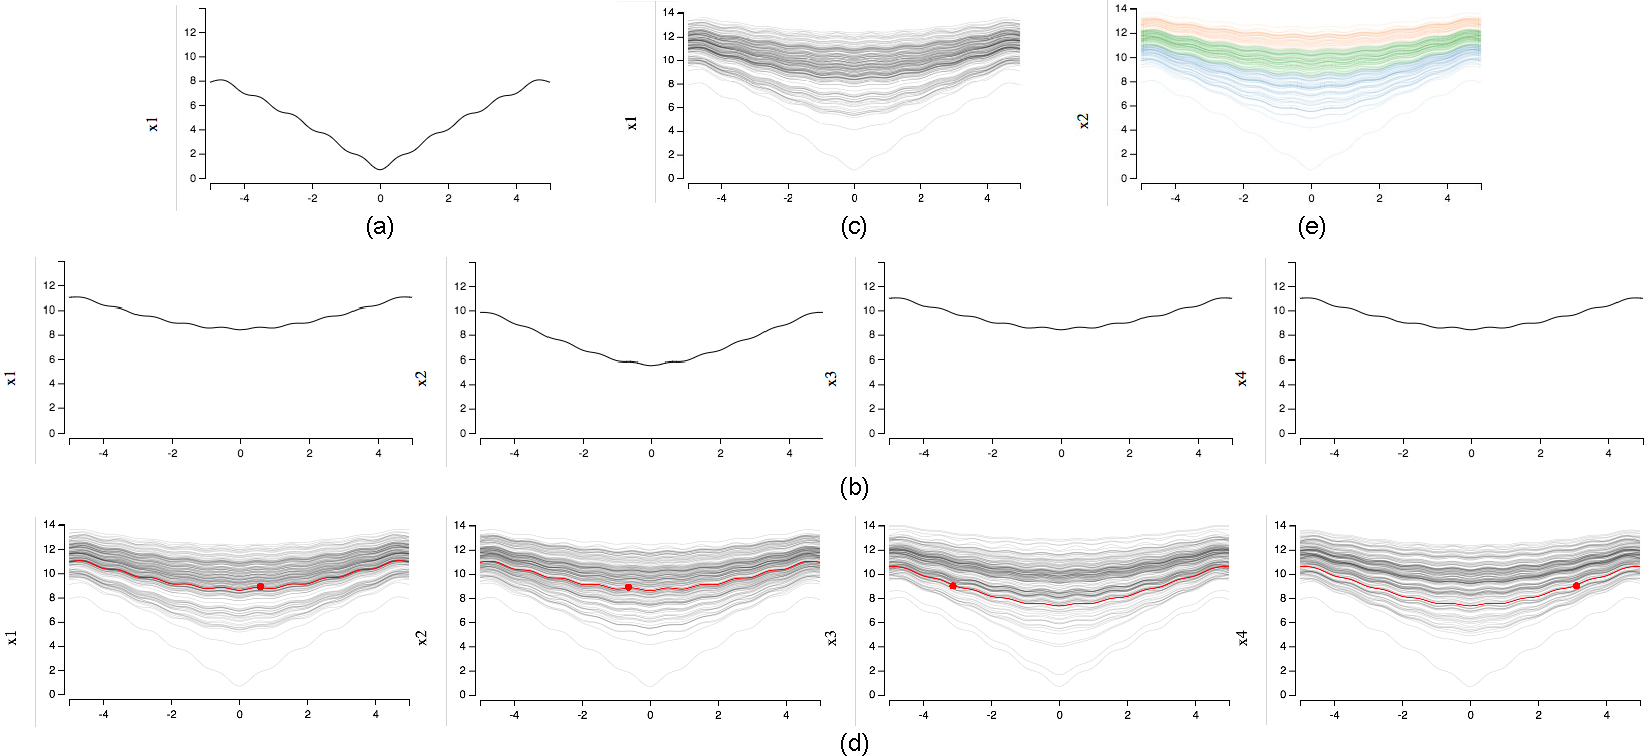
\includegraphics[width=0.9\textwidth]{sliceplorer_overview.pdf}
  \caption[The evolution of Sliceplorer.]{%
    The evolution of Sliceplorer. I adapt the commonly known technique of
    1D function plots (a) to
    multiple dimensions by taking a small multiples approach and repeating each
    plot for each dimension (b). I address the
    focus point selection problem by sampling over the parameter space and then
    projecting the slices in the corresponding plot
    (c). The user can mouse over a particular
    slice in one plot and the corresponding slices are highlighted in the other
    dimension plots (d). This allows one to
    see the corresponding function behaviors in the other dimensions.  Finally,
    one can cluster the function slices (e), to
    show groups of similar behavior in the manifold.
  }
  \label{fig:walkthrough}
\end{figure}

First, we turn to the visual exploration of multi-dimensional continuous
functions. In this case, the user is primarily interested in the relationship
between dependent and independent variables. In this chapter, I discuss how
one-dimensional slices can be a highly intuitive way of visualizing
multi-dimensional manifolds. I also discuss how we can use projections of 
slices to address the focus point selection issue. The task analysis in this
chapter introduces manifold analysis tasks.
This chapter was based on work published as \bibentry{Torsney-Weir:2017a}.


%Thesis: Multi-dimensional spaces are better visualized through slice based views

We live in a three-dimensional world.  Ourselves and what we can interact with
are in three dimensions.  We learn about our world by studying the various
phenomena around us.  These phenomena are described as continuous processes.
In the beginning of our  education we study function plots in high school.
These give an intuitive view of one-dimensional phenomena.  By exploring the
relationship between an input factor
and output,
we can build an understanding on the relationship between the two.  We can also
compare one function plot to another. Visual inspection of these plots allows
us to see common patterns. We use our pattern recognition ability to quickly
categorize these different plots into different types of function behavior.
Function plots can also be used to describe two-dimensional phenomena. These
show the effect due to two input factors. In this case we can use the third
dimension or color encoding to show the function value.  From these plots we
can also make general statements about the ``shapes'' of the behavior like how
``peaky'' the function is or if it is monotonically increasing. These shapes
give us intuition into the underlying processes and help us learn about the
world~\cite{Palmer:1999}.

We also interact with many phenomena around us that are essentially
multi-dimensional in nature. For example, the weather in a certain location is
determined by the temperature, pressure, humidity, dew point, wind velocity,
and wind direction, among others. A change in any of the factors results in a
change in the weather. Each of these factors can be given a ``spatial
embedding.'' Then, they can be viewed as a dimension of some space.  By
``walking'' or navigating through this space we can observe the effect on the
weather due to changes in these parameters. 

Understanding multi-dimensional continuous spaces is difficult. As
three-dimensional beings we have real-world analogs for measurement, angle, and
position in three dimensions. We do not have these once we move beyond three
dimensions though. Nevertheless, visual analysis of these multi-dimensional
spaces has produced insights about the underlying
behavior~\cite{Sedlmair:2014,Gleicher:2016}. The issue is how to show more than
three dimensions on a two-dimensional screen. 

One strategy is to discretize the dataset through sampling and then use the
wealth of discrete visualization tools available. Much of the work on
multi-dimensional data analysis developed from analysis of 
tabular data. These datasets are often recorded from real-world
events such as census, species, or text data and contain many different aspects
about each entity. Thus, these datasets are inherently multi- or high-dimensional.
Each different aspect of the data items creates a dimension to be analyzed. 
In the case of these data the mental model is that of discrete objects
like humans, plants, or documents. Since the mental model is discrete in this
case it makes sense to use data processing and visualization tools designed for
discrete data.  However, our mental model for physical data is a continuous 
one. Therefore, the
discrete data paradigm breaks our mental model~\cite{Tory:2004a,Liu:2010a}. 
Breaking the mental model means that the visualization is not conveying the
complexities of the continuous phenomena.
Rather, we
should use visualization techniques purpose-built for continuous data.

While not as
extensively developed, there is previous work on visualizing multi-dimensional,
continuous data. These techniques can be broadly classified into projection,
topological, and slicing methods.  
Projection methods attempt to
distort the multi-dimensional object in order to view it on a two-dimensional
screen. With projection techniques we can preserve distance, direction, size,
or angles, but not all of 
these~\cite{Snyder:1987}. 
Depending on the
projection method, we may see radically different representations.  The issue
is that it is not clear from the resulting visualization what sort of
transformation was performed on the data.  Thus it can be difficult to
reconstruct the mental model of the multi-dimensional object.  One of the most
often seen multi-dimensional projection techniques is the Schlegel
diagram~\cite{Sommerville:1929} which picks a ``face'' of a polytope and projects the
remaining faces inside it. Thus, this technique only works for 4D polytopes.
Topological methods search the continuous dataset for values of interest, such
as critical points or contours.  Topological visualization techniques also
suffer from the issue of unclear transformation. It is difficult to relate the
resulting visualization back to features in the multi-dimensional object.

Slice-based views of multi-dimensional continuous spaces have not been explored
as extensively as other options.  This work began with the advent of
HyperSlice~\cite{Wijk:1993}.  HyperSlice extends the idea of slicing from
medical imaging to any number of dimensions.  HyperSlice provides the framework
for visualizing multi-dimensional continuous objects as a set of
two-dimensional slices.  There are $d \choose 2$ subpanels, one for each pair
of dimensions. Each panel shows a 2D slice of the object. The horizontal axis
shows one dimension and the vertical axis shows another dimension. Essentially,
each sub-plot of HyperSlice shows a 2D function plot. With 2D slices of solid
multi-dimensional objects color is often used to encode value. 

My work is inspired by the HyperSlice technique. Van Wijk and van Liere
introduced the idea of using slice-based views of multi-dimensional data.
However, they did not expand on what data types and tasks are involved in
multi-dimensional continuous data analysis.  I build on their work,
investigating the usefulness of slice-based views of continuous
multi-dimensional datasets. I also identified tasks involved in
multi-dimensional data analysis. The task analysis informed the development of
one- and two-dimensional slice-based views.

In this thesis I will explore
the possibilities of these slice-based views. Through a number of case
study examples, I will demonstrate the power of these views and ways to
address their shortcomings.

\subsection{Multi-dimensional spaces}
\label{sec:motivation:multi-d}

There are a number of domains where one can apply the analysis of continuous
multi-dimensional data.  As of yet, there has not been a comprehensive data and
task analysis for multi-dimensional continuous data analysis. For discrete
data, there are several task 
analyses~\cite{Shneiderman:1996,Brehmer:2013,Amar:2004}. 
However, they are
focused on identifying and selecting particular data items. Continuous datasets
consist of ranges of values as well as functions. Functions can be seen as a
mapping from ranges of numbers to other ranges. The analysis task here is to
study these ranges, their relationships to each other, and the mappings between
them. Tasks addressing these
have not yet been covered by visualization task analyses. Thus,
there is no comprehensive source for what analysis tasks one wants to perform
given a continuous multi-dimensional dataset.  Work in this area has
traditionally focused on developing a specific visualization for a specific
task. For example, topological spines extracts critical points from a scalar
field~\cite{Correa:2011}. One goal of this thesis is to develop this task
taxonomy for visualization of continuous multi-dimensional data.


These domains can be broadly classified into two types based on their analysis
tasks. One type, \emph{manifold} analysis, deals with understanding the
relationship between inputs and outputs. This is a functional relationship.
The user wants to inspect how changes in the inputs (independent variables)
affect the outputs (dependent variables). One can also perform \emph{shape}
analysis. Here, in terms of the analysis tasks, there is no identification of
independent and dependent variables. We look at each of these two in turn.

\subsection{Manifolds}
\label{sec:manifolds}

Studying the mapping between continuous ranges means studying functional
relationships and thus manifolds.  The critical issue is understanding the
relationship between independent and dependent variables.  Subtasks in manifold
analysis include examining critical points, assessing the sensitivity of
parameters, and understanding the shape of the manifold.  
One area where
understanding the manifold is important is analyzing optimization surfaces and
functions.  In this case, the identification of extrema is important for
understanding how many and the relative location of local optima. In addition,
we want to understand the degree to which these are extrema. These can result
in global optimization algorithms ``getting stuck'' in local optima rather than
continuing to search for the global optimum. Optimization algorithms need to be
carefully tuned to properly detect these features and ignore them where
necessary.

Simulations can be used to run experiments that are impractical or impossible
in the real world.  Simulation analysis is another area where the analysis
tasks, in the abstract, are examining functions. If we look back at the weather
simulation from before, the inputs to the function are things like the
temperature and pressure.  The output is, for example, the likelihood of rain
the next day. The function is the simulation itself. Computer simulations are
deterministic.  A deterministic simulation has a fixed mapping from each unique
input parameter configuration to an output value. This is the same as a
functional relationship. The sensitivity and extrema are also important to
simulation analysis.  Thus, these can all be analyzed with visualizations of a
manifold.

To date, manifold visualizations have concentrated on a particular analysis
task or a particular application domain. For example, visualizations of the
Morse-Smale complex~\cite{Gerber:2010} are focused on showing only critical
points of the manifold. As with any visualization designed for a specific task,
they must be used in combination with other views for visual analysis of
domain-specific data. Domain-specific visualizations often used linked views to
show different aspects of data to accomplish multiple tasks at once. However,
they are purpose built for a specific domain. While techniques may transfer
from one domain to another~\cite{Sedlmair:2012}, it is not always clear how.
My goal is to unify these methods to a certain extent.  As I will show in
\autoref{chp:sliceplorer}, slice-based views of manifolds can be used for a
wide variety of tasks in a wide number of domains.

\subsection{Shapes}
\label{sec:shapes}

One may also want to understand the relationship or correlation between
multiple continuous values. In the manifold analysis case we have the notion
of independent and dependent variables. This classification does not exist 
here.
In this case
we want to study the relationship of all variables. Careful study of the shape
of the dataset can give insight into the relationship between the various
ranges of dimensions of the object. For example, one may want to know if the
overall shape is a sphere, donut, or box. In addition one may be interested in
any kinks or cusps in the dataset. Changes in the gradient and curvature of
the shape are also of great interest. These indicate changes in correlation or
relation.

The analysis tasks of multi-dimensional shapes can be applied to a number of
different areas. The study of polytopes is one such area and perhaps the most
direct application of understanding multi-dimensional continuous shapes.
Polytopes are the multi-dimensional generalization of polyhedra and polygons.
The tasks are to understand the symmetries and patterns making up the
polytopes~\cite{Ziegler:2012}. Perhaps a less obvious connection is the
analysis of the tradeoff curves in multi-objective optimization. Since we are
performing optimization we are interested in the tradeoffs amongst all the
non-dominated points~\cite{Kung:1975}. This is also known as the Pareto
front. In this case, the user wants to understand what are the costs of
reducing one or more parameters in order to increase the value of others. Cusps
or large changes in curvature in these datasets are important since they show
critical changes in the rate of tradeoff.  With a proper view of a
multi-dimensional object we can also view differences between two objects
directly. 

These two different data types and sets of tasks require different visualization
considerations. Proper visualization for manifold analysis should focus on
the relationships between independent and dependent variables. Visualizations
of shapes do not have this mapping requirement and instead focus on the 
relationships between dimensions. With this categorization in mind, we can now
examine the available visualization techniques to examine these.


\subsection{Visualizing multi-dimensional continuous spaces}
\label{sec:multi-d-challenges}

Understanding multi-dimensional space is difficult. As humans, we simply do not
have the spatial analogs in more than three dimensions. A number of methods
have been developed to extract specific features from the multi-dimensional
object. For example, when studying polytopes, the number of faces and
symmetries is very important~\cite{Ziegler:2012}. However, these only produce
an answer without sufficient context. They do not necessarily give any
intuition as to how to transfer our three-dimensional knowledge to
multi-dimensional spaces.

Visualizations of multi-dimensional spaces on a 2D screen must contend with
some sort of reduction of the information. A proper visualization must select
visual encodings that highlight the information we want to see. Any sort of
data reduction requires trade-offs. The best visualization choices acknowledge
any deficiencies to a particular visual encoding. By acknowledging these
deficiencies, we can design tools to compensate for their shortcomings while
still maintaining their advantages. Therefore, it is worth first looking at the
possible mappings of data to visual elements. Then, I present commonly used
visual encodings of multi-dimensional continuous data using these mappings.

\subsection{Encoding multi-dimensional data}

Multi-dimensional continuous data consists of a set of continuous ranges, one
for each dimension. In the case of manifold analysis, each of these ranges can
be additionally classified as ``dependent'' or ``independent'' depending on
which side of the mapping they are on. Typical visualization practice is to
give each dimension a separate visual channel. There are a number of possible
visual channels that have been identified.  The ranking of effectiveness of
visual channels (shown in \autoref{tbl:visual_encodings}) was proposed by
Bertin~\cite{Bertin:1967} and confirmed through experiments by Cleveland and
McGill~\cite{Cleveland:1984}, Mackinlay~\cite{Mackinlay:1986}, and Heer and
Bostock~\cite{Heer:2010}.  Munzner~\cite{Munzner:2014} provides a summary of
the results. We are also limited in how many channels we can use
simultaneously. According to Ware~\cite{Ware:2004}, certain channels, such as
red and green are not visually separable. 

\begin{table}
  \caption{Rankings of visual encodings of quantitative data}
  \label{tbl:visual_encodings}
  \begin{adjustbox}{max width=\linewidth}
  \begin{tabular}{llll}
    Bertin~\cite{Bertin:1967} & Cleveland and McGill~\cite{Cleveland:1984} & Mackinlay~\cite{Mackinlay:1986} & Munzner~\cite{Munzner:2014} \\
    \hline \\
     Position & Position along a common scale & Position & Position on common scale \\
     Size & Position along identical, nonaligned scales & Length & Position on unaligned scale \\
     (Grey) Value & Length & Angle & Length (1D size) \\
     Texture & Direction & Slope & Tilt/angle \\
     Color & Angle & Area & Area (2D size) \\
     Orientation & Area & Volume & Depth (3D position) \\
     Shape & Volume & Density & Color luminance\\
     & Curvature & Color saturation & Color saturation \\
     & Densities & Color hue & Curvature \\
     & Shading & & Volume (3D size) \\
     & Color saturation &           & 
  \end{tabular}
  \end{adjustbox}
\end{table}

The difficulty of visualizing a continuous multi-dimensional space on a
two-dimensional screen brings a number of challenges. We treat each dimension
separately, thus, we need several different visual channels. However, there are
simply not enough visual channels available to draw a 15-dimensional object in
a single view. This is further complicated by the fact that separate visual
channels are not necessarily visually separable.  Furthermore, each dimension
of the multi-dimensional object under study is treated equally. For example, no
particular axis of a polytope is more important than any other.  We should
encode each dimension using equally weighted effectiveness channels.  With
fewer channels available than data dimensions we either need to reduce the data
or use multiple views to properly visualize the data.


\subsection{Methods}

The common taxonomy of how to view multi-dimensional data on screen is based on
discrete data analysis. There, there are two categories: dimension reduction or
projection. With continuous data, though there is a third possibility, that of
slicing. Therefore, I view the taxonomy of \emph{continuous} multi-dimensional
data analysis methods into two categories. Data-driven methods include both
projection and dimension reduction and reduce the dimensionality of the data
before visualization. View-based methods reduce the data during the
visualization. Slicing is a view-based method.

Purely data-driven methods are commonly known as feature selection or dimension
reduction. The goal is to find a subset of dimensions that are critical to
understanding the dataset. Topological techniques take this a step further.
They discard all spatial information about the dataset and only concentrate on
the difference in function value, as in the Morse-Smale
complex~\cite{Gyulassy:2012a}, or evolution of contours, as in the contour
tree~\cite{Carr:2003a}.  Projections also synthesize the dataset into new
dimensions to show using visual channels. Principal component
analysis~\cite{Holbrey:2006} is a popular choice in this area. This rotates the
space and thus produces new set of dimensions that are a linear combination of
the input dimensions. Even this relatively simple operation (a rotation) can be
difficult to understand. For example, iPCA~\cite{Jeong:2009a} was a tool to
help users understand the effects of the dimensional transformation.

View-based methods try and produce multiple linked views of a multi-dimensional
dataset from different angles. Each view shows a subset of the dimensions.
This way we can use a proper set of visual channels for each view.  We use
interaction to link these different views. These multiple, coordinated, linked
views have been one of the biggest success stories from the visualization
community~\cite{Rao:1994}. The traditional HyperSlice~\cite{Wijk:1993}
technique falls into this category. Each panel of the HyperSlice view shows two
of the input dimensions and the value is encoded with color.
The views are linked through the focus point selection. Changing the focus point
in one sub-plot updates the other sub-plots.

My work focuses on the exploration of the combination of data-driven and
view-based methods.  Data-driven methods reduce the data in a way that we can
get a global overview of the dataset. View-based methods are much more detailed
but can only produce a local view of the data. By combining these methods I can
achieve both a global overview as well as an on-demand local view of the
dataset in a single visualization. 


\subsection{Slices}
\label{sec:slicing-advantages}

Slicing offers a number of advantages over other multi-dimensional
visualization techniques. Slicing is a direct visualization of the
multi-dimensional object. In contrast to methods like projection or dimension
reduction, slicing does not distort the dimensions in order to display them on
a two-dimensional screen. Since there is no distortion, distances in the visual
representation are directly proportional to distances in the object. This is
one of the reasons that slicing is popular in the medical imaging community.
Sizes of organs or tumors can be measured visually on screen. Additionally,
relative sizes correspond to what a doctor would expect to see in the body.
Multi-dimensional data is abstract. It lacks the correspondence to real-world
objects that the medical community uses to understand their two- and
three-dimensional datasets. Nevertheless, it is still important in
multi-dimensional data analysis to properly estimate distances and relative
sizes. 

Another benefit of the direct visualization is that users do not require
extensive training to understand the visualization. The concept of slicing
through a three-dimensional object is a familiar one. Humans are used to this
even from slicing fruits and vegetables with a knife. This concept of slicing
can be extended from this well-known metaphor to cover multiple slices of
multi-dimensional objects.

Slice views use the horizontal and vertical axes for showing the effects due to
the input parameters. These axes are the most perceptually
uniform~\cite{Stevens:1957} and are considered the most effective
(\autoref{tbl:visual_encodings}). One- or two-dimensional
plots are replicated for each combination of dimensions in order to show more
than two dimensions at once. This promotes familiarity of the visualization.
Once the user has learned to read a single panel, they can apply this knowledge
to the remaining panels. This approach follows the principal of small
multiples~\cite{Archambault:2011}. 

In order to produce a slice plot one needs to first pick a particular
\emph{focus point} in the multi-dimensional space. This focus point determines
which slices are being viewed. Selecting a good focus point a-priori is
difficult. 
It either requires a great deal of luck or careful analysis of the
dataset. This is not always possible. Slice-based views require some sort of
interactive focus point selection. Interactively browsing through the slices
requires interaction controls to give the user control over the focus point.
Furthermore, we need some kind of navigation map to show which focus points the
user has selected so that they do not become lost. Neither of these navigation
aids are well developed at this point. This need for interaction is likely one
of the reasons that slice-based views have not developed as much as projection
or topological techniques. Static views are much easier to include in papers
and don't require explanation prior to use.

The other implementation issue of slice-based views is ensuring that the
visualization can remain interactive. In this case, interactive is defined as
the rate at which the user can maintain their
concentration~\cite{Shneiderman:1987}. This is often defined at 10 frames per
second. It can be difficult to compute a 2D slice of an arbitrary complex
multi-dimensional object. 


\subsection{Upcoming}
\label{sec:thesis_outline}

My goal is to highlight the advantages of slice-based methods for
multi-dimensional data analysis. At the same time I want to address the
limitations. The end goal is to bring slice-based views into the standard
toolbox of visualizations.

In \autoref{chp:sliceplorer}, I examine how to visualize manifolds using
slices. I present Sliceplorer which is a system to view one-dimensional slices
of multi-dimensional manifolds. I use projections of these one-dimensional
slices instead of showing one focus point at a time. I also go into detail
about the tasks one wants to perform with manifold analysis.

I extend the idea of projections of slices to the second dimension in
\autoref{chp:hypersliceplorer}.  I show how this can be used to effectively
visually analyze the shape of multi-dimensional data. In many cases, this data
is given as a simplical mesh. I introduce an algorithm to compute 2D slices of
this mesh.  Using this algorithm, I show how we can visually understand
datasets like Pareto fronts or polytopes.

Finally, in \autoref{chp:rendering}, I discuss how we can take advantage of the
multi-dimensional geometry and GPU architecture to allow interactive-speed
browsing of the focus points. In addition to this algorithm, I develop a method
that can predict the amount of time needed per element to draw one frame of the
visualization. I then show how this estimation formula can be calibrated to a
particular user's hardware.



\section{Related work}
\label{sec:related-work}

Multi-objective optimization and multi-dimensional objects are two areas
where it is important to study shapes in over three dimensions. We discuss 
these areas below. Topological techniques are based on viewing critical points
of manifolds~\cite{Correa:2011,Gerber:2010} or how contours merge and 
split~\cite{Carr:2003a}. We do not discuss them further. Manifold analysis
is very different than visualizing shapes. 

The need to understand multi-dimensional polytopes is apparent to 
geometers~\cite{Ziegler:2012}.
However, there are a number of cases in computational science where the
understanding of the size and the shape of a sub-section of the parameter space
is of importance~\cite{Bergner:2013,Sedlmair:2014}. One of these cases is
highlighted in \autoref{sec:bernstein}. Another use case is the study
of multi-dimensional Pareto fronts (\autoref{sec:pareto}).

\subsection{Multi-objective optimization}

In multi-objective optimization we have several scalar values that we wish to
optimize. The set of optimal points is known as the Pareto front.
If each objective measure is continuous then we have a continuous hull in one
orthant. We want to use this hull to analyze the trade-offs between objective
measures. Interactive decision maps~\cite{Lotov:2004} show a 3D Pareto front as
a series of 2D slices. Any objectives past three must be constrained to a value
however. Objective functions are difficult to sample since we often do
not have control over the sampling of the range of a function.  To
generate this hull one often samples the objective functions and then computes
the Pareto points using an algorithm such as NSGA-II~\cite{Deb:2002} or the
skyline algorithm~\cite{Borzsony:2001}. We can then generate the hull using
multi-dimensional marching cubes~\cite{Bhaniramka:2000}, the quickhull
algorithm~\cite{Barber:1996}, or alpha shapes~\cite{Edelsbrunner:1983}. These
can then be viewed in Hypersliceplorer as we do in \autoref{sec:pareto}.

An alternative is to treat the samples as a fixed set and then visualize the
relationship between possible combinations of objectives. Typically this is
done by examining the weight space through interaction. 
LineUp~\cite{Gratzl:2013} uses a ranked list approach and shows the user
how rankings will change as the user changes the relative weighting for each
objective. WeightLifter~\cite{Pajer:2016} extends this by also showing the
stability of rankings. The user can understand how much a particular objective
is affected by its weighting. This can help speed interactive exploration. 
Finally, the joint contour net~\cite{Carr:2014} can be used to compute how
often two objectives hold particular values simultaneously. 
In our case, the mental model is a continuous one. Thus it makes more sense
to show a continuous Pareto front.

\subsection{Multi-dimensional objects}

%TM: I wanted to add a sentence like this, but I dont think we need to after all: Since we are focusing on the visualization of continuous objects in multiple dimension, literature on projection based techniques is not relevant and will not be mentioned. 

%We review related work on the visualization of multi-dimensional continuous objects.

When speaking of 3D polytopes, their source is usually either from reconstruction of 3D point clouds 
(see Dey~\cite{Dey:2006})
or from iso-surfacing techniques (see Wenger~\cite{Wenger:2013}).
%However, we believe that the method of choice for visualization of 3D shapes are 3D renderings.
%Visualization of (continuous) objects in three (or fewer) dimensions is not that relevant for our discussion, since we believe that our method will not be of advantage here. Still, in the are of volume visualization there are quite a wealth of approaches for creating an iso-surface, which creates a 3D polytope. See also the excellent text books by Wenger or Day
%
%often falls under the name of
%volume visualization.  Three-dimensional volumes can be rendered using
%techniques isosurface techniques like marching cubes~\cite{Lorensen:1987a} or direct volume visualization. 
There are extensions to iso-surfacing techniques in multiple dimensions~\cite{Bhaniramka:2000}, 
%Marching cubes has been extended to arbitrary
%dimensions 
but in more than three dimensions we must distort the space somehow to visualize the object. 

For the visualization of 4D polytopes, there are a number of techniques for moving from four to three dimensions.  The
Schlegel diagram~\cite{Sommerville:1929} is one such method based on
projection. We pick a face of the figure, usually the largest, which is a
three-dimensional object. Then, all other faces are ``packed'' inside this face in
such a way that we can show the connections between faces. The Schlegel diagram
works well for regular polytopes where we have some previous intuition about
the faces. However, for an arbitrary simplical mesh, any face is a simplex
which we need to project into. All Schlegel diagrams of a simplical mesh look
like a simplex with a number of other simplices inside them. It can be
difficult to recover what the original object looks like because the
cross section is lost. An alternative approach is to treat the fourth dimension
as time and then produce an animation of the evolution of the shape in three
dimensions. In this case each frame of the animation is a 3D slice of the 
object. Rather than first projecting from 4D to 3D and then rendering the
projection, Hanson and Cross~\cite{Hanson:1993} propose a method to first
render the object in 4D and then view the three-dimensional projection. This
allows them to show unique lighting effects from the 4D surfaces.
%One can also use a stererographic projection. 
As with all projection methods, if the user is unaware of the details of the
method it can be difficult to build a mental model of the shape under study.

Hasse diagrams~\cite{Battista:1988} are based on showing the connectivity
between vertices of an object. These can be seen as network diagrams where the
vertices of the figure are the nodes in the graph and the edges of the graph
are the edges in the figure. These have a number of layout issues.  For visual
understanding, humans prefer a 2D planar graph~\cite{Kieffer:2016}. Good layouts
of the Hasse diagram must balance human aesthetic needs like few edge crossings
with the geometric interpretation. 
There are automatic layout
algorithms, such as the one by Battista et al.~\cite{Battista:1988}, but these
do not work in all cases.

For more than four dimensions, 
projection methods no longer work as well.  Techniques based on slicing the
space can be extended to any number of dimensions.  The techniques to perform
this so far, such as HyperSlice~\cite{Wijk:1993},
HyperMoVal~\cite{Piringer:2010}, and Sliceplorer~\cite{Torsney-Weir:2017a},
are designed to show slices of multi-dimensional manifolds.
They produce slices by
constraining all but two (for 2D slices) or one (for 1D slices) of the
dimensions to the focus point value and then producing a heatmap, contour plot,
or function plot. Sliceplorer addressed the focus point issue by sampling over
a number of focus points and projecting them down.  Exploded view
diagrams~\cite{Karpenko:2010} offer a hybrid method between a 3D volume
visualization and slicing.  However, they 
%also require a parametric description of the object under study and 
are limited to 3D objects. 
The global view of Hypersliceplorer is inspired by the idea of examining
cross sections. We also have a local
view which permits the user to look at a small number of self-selected slices.
We have developed a method to produce slices based on a simplical mesh which
is very useful given a discretized surface (see \autoref{fig:slicing}). 


\section{Sliceplorer}

When developing our technique, we first identified design requirements with
respect to tasks that a user would perform when analyzing multi-dimensional
scalar functions. We continuously evaluated how our technique fits with these
requirements and iteratively adapted it to encompass as many tasks as possible.
A static slice view itself does not address many of the tasks required so we
use interaction methods to address these and create a comprehensive technique.  

\subsection{Design requirements}

When analyzing a function visually, there are a number of features that the
user wants to see.

\textbf{R-peaks}: The most obvious feature
is identifying peaks and valleys. This is primarily done to find the
global optimum of a function. 

\textbf{R-robust}: The relative height
around each optima is important to detecting the robustness of that optimum. In
some cases one may prefer a local optimum over a global one if it is more stable.
%\ttwnote{there is SA, but visual analysis gives context} 
This is very common in
simulations of manufacturing processes where variations in manufacturing tolerances
should not affect the performance of a part too much~\cite{Berger:2011}.  
%\tmnote{should we site berger11 again?}

\textbf{R-bowl}: Similarly, we may be
interested in how ``bowl''-shaped the area around an optimum is. The goal is
similar to robust optimization but rather than looking for ``flat'' areas of
the function we are looking for areas with smooth gradients. The amount of this
smoothness is important for correctly parameterizing optimization
algorithms~\cite{Back:1996}. An incorrect parameterization can either cause them to
get ``stuck'' at some local minimum or make unreasonably slow progress towards
the global minimum. 

\textbf{R-overall}: Finally, we want to view the overall ``shape'' of the
function. It is important to understand if it is smooth everywhere and how much
variance there is in the function. When building a surrogate regression model
we need to know if the function has consistent variance and we need to choose a
model that captures this behavior. 

All of
these requirements mean that we need to view more than just the maxima and
minima of a function.
%\ttwnote{we need to look because there's no clear objective}

\subsection{Intuition}

If we were analyzing one-dimensional continuous functions then the choice would
be obvious: a line plot like the one in \autoref{fig:walkthrough}a. The x-axis
is used for the independent variable or parameter setting and the y-axis is
used for the dependent variable or scalar value of the function. The function
response is shown with a line. This is a metaphor that anyone who has taken
high-school algebra can comprehend. The vertical and horizontal location
channels visually encode the primary values of interest. These are the ``best''
visual channels to use in terms of accuracy and sensitivity to differences
according to Bertin and others~\cite{Bertin:1967, Mackinlay:1986}. 

We show the evolution
of our technique from a one-dimensional function to the full multi-dimensional
Sliceplorer view in \autoref{fig:walkthrough}. 
To extend this simple technique to multi-dimensional functions we simply repeat
the one-dimensional function plot for each parameter
(\autoref{fig:walkthrough}b). 
We will have \(d\) plots where \(d\) is
the number of dimensions in the function. In the same way that
HyperSlice~\cite{Wijk:1993} is inspired by the SPLOM layout, we can use any
layout technique for multiple histograms. 2D slices scale as $\mathcal{O}(d^2)$
which is worse than the $\mathcal{O}(d)$ for 1D slices. 
1D slices also give us separable channels remaining for encoding of additional
information such as uncertainty or optimization traces (see
Sec.~\ref{sec:optimization}).

Slicing offers a number of advantages over projection-based views like
scatterplots and histograms. Slices give context around a particular focus
point. We can see the precise shape of the function at this point.  For
example, peaks and valleys (\textbf{R-peaks}), flat areas (\textbf{R-robust}),
and variance in the function can all be seen directly.  While scatterplots and
histograms can be used to see general trends, they suffer from ``false
distances'' where points that are visibly close to each other are not actually
close to each other. 

\subsection{Focus point projection}

Showing a local 1D slice requires the selection of a single focus point, i.e.\
a point in multi-D through where all 1D slices intersect. Once this focus
point is selected, we can use an off-the-shelf 1D function plot drawing
method to draw the slice itself.
Rather than only
showing one focus point (i.e.\ one slice line per dimension) at a time and
having the user choose a focus point we select multiple focus points
automatically. This enables a more global view of the function
(\textbf{R-overall}). Now, all 1D slices (one per focus point and dimension)
are projected onto the same plot (see \autoref{fig:walkthrough}c).  In doing
so, users do not need to memorize the previously seen slices, they can look
among them to see general trends. This approach combines the ideas of slicing
and projection, and fosters one of the core strengths of visualization:
``perception beats recall''~\cite{Munzner:2014}. 

We are using a Sobol sequence~\cite{Sobol:1967} to select the focus points
themselves.  The Sobol sequence is a space-filling, quasi-random,
low-discrepancy sequence that is designed for sampling in high dimensional
spaces.  The Sobol sequence will give us a sampling of the multi-dimensional
parameter space with an economy of samples. This will maximize the chances that
we will see extrema (\textbf{R-peaks}), plateaus (\textbf{R-robust}), and bowls
(\textbf{R-bowl}) in our 1D slices.  In addition, using a Sobol sequence makes
it easy to adjust the number of 1D slices shown (i.e.\ focus points) on the
fly.  Specifically, it avoids a complete resampling of the parameter space like
we would need with a Latin hypercube sampling. 

%The number
%of focus points is user-adjustable so if they want to see more or fewer numbers
%of sample points they can. \msnote{this goes into details now. Imho what is
%missing before is a good high-level summary of what our technique is actually
%doing. There is the N plots things, but not the sampling thing, nore the
%overdrawing. A good mental model would at the beginnign would be really cool
%... maybe this was in the intro and I just forgot :)}


\subsection{Linked selection}

One disadvantage with 1D views over 2D views is that we cannot see the
two-dimensional interactions anymore. We compensate for this with
interaction. %\msnote{should comparisons to other VE techniques, 2D slices, topology, be here or in a section further down? ... hmm just a thought ... maybe both is fine if we only have it short here ...}
The user can mouse over a particular slice which will highlight
all slices corresponding to that focus point. That is, one slice in each view is highlighted.
We also superimpose the focus point itself on these lines. In doing so,
the user can see the behavior of the function with respect to the other
parameters around that focus point (see \autoref{fig:walkthrough}d).

\subsection{Clustering}

\begin{figure}
  \centering
  \begin{subfigure}[b]{0.48\columnwidth}
    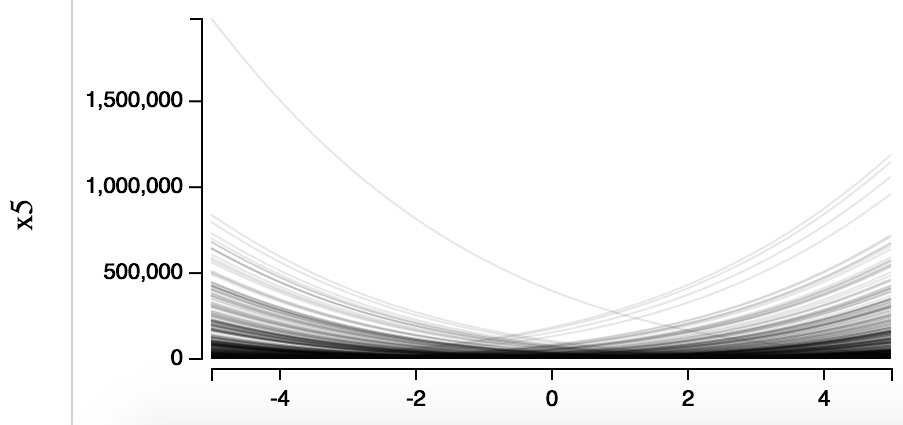
\includegraphics[width=\textwidth]{zakharov_confusing_unclustered.png}
    \caption{
    }
    \label{fig:cluster:none}
  \end{subfigure}
  ~
  \begin{subfigure}[b]{0.48\columnwidth}
    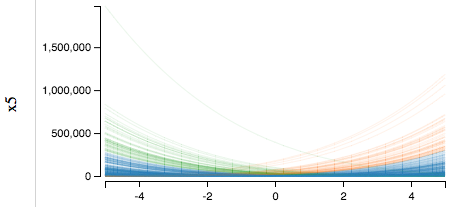
\includegraphics[width=\textwidth]{zakharov_color_clusters.png}
    \caption{
    }
    \label{fig:cluster:clustered}
  \end{subfigure}
  \caption{
    500 projected slices of the 5th dimension of the 5D Zakharov~\cite{Back:1996} 
    function. It is difficult to see if the slices are bowl shaped or two sets
    of monotonically decreasing and increasing curves. It is much clearer in 
    the cluster view that there are actually three sets of curves: 
    there is a set of monotonically decreasing curves and a set of 
    monotonically increasing curves. The very low-value curves form a third
    set.
  }
\end{figure}

Similar to visual encoding techniques such as parallel coordinate plots, projected 1D slices might mask certain patterns due to
overdrawing.
\autoref{fig:cluster:none} is an example where it is difficult to tell if the
slices are monotonic or bowl-shaped (\textbf{R-bowl}). The interactive slice highlighting
can give some insight into how individual slices are behaving but lacks
a global method to distinguish groups. We offer a
clustered slice view to address this (\autoref{fig:cluster:clustered}). 
The clustering is done with a k-nearest neighbor algorithm using the
$L^2$ distance between two slices as the distance metric.
This allows us to group the slices into distinct
groups of behavior and color-code these groups to distinguish them.

%These methods overcome many of the limitations of showing slices as
%compared to projection or topological methods while retaining the
%benefits. \msnote{hmmm ... coming back to my point from above: wouldn't it be good to first show that the general idea is good/better than STAR in certain cases before speaking of overcoming its limitations ... maybe this is just a framing issue ... }


\section{Task-based evaluation}
\label{sec:task-eval}

\definecolor{key0}{RGB}{242,240,247}
\definecolor{key1}{RGB}{203,201,226}
\definecolor{key2}{RGB}{158,154,200}
\definecolor{key3}{RGB}{106,81,163}
\newcommand\crule[1]{\textcolor{#1}{\rule{7pt}{7pt}}}

\begin{table*}[t]
  \centering
  \caption[Summary of the task-based evaluation]{%
    This table shows the summary of the task-based evaluation. I extended the discrete 
    data-focused tasks of Amar, Eagan, and Stasko~\cite{Amar:2005} to directly address
    continuous data, with the exception of ``sort'' (see \autoref{sec:task-eval}). 
    The table shows the scores from our qualitative results inspection as well as
    the expert study on a scale from
    ``none''~\crule{key0}, ``partially''~\crule{key1}, ``mostly''~\crule{key2},
    to ``fully''~\crule{key3}
    where
    ``none'' means that the task is not addressed at all and ``fully'' means 
    that this
    task is directly supported by this view. There are quotes of
    the general description from Amar, Eagan, and Stasko's paper in the ``discrete''
    column for reference. 
  }
  \label{tbl:task_list}
  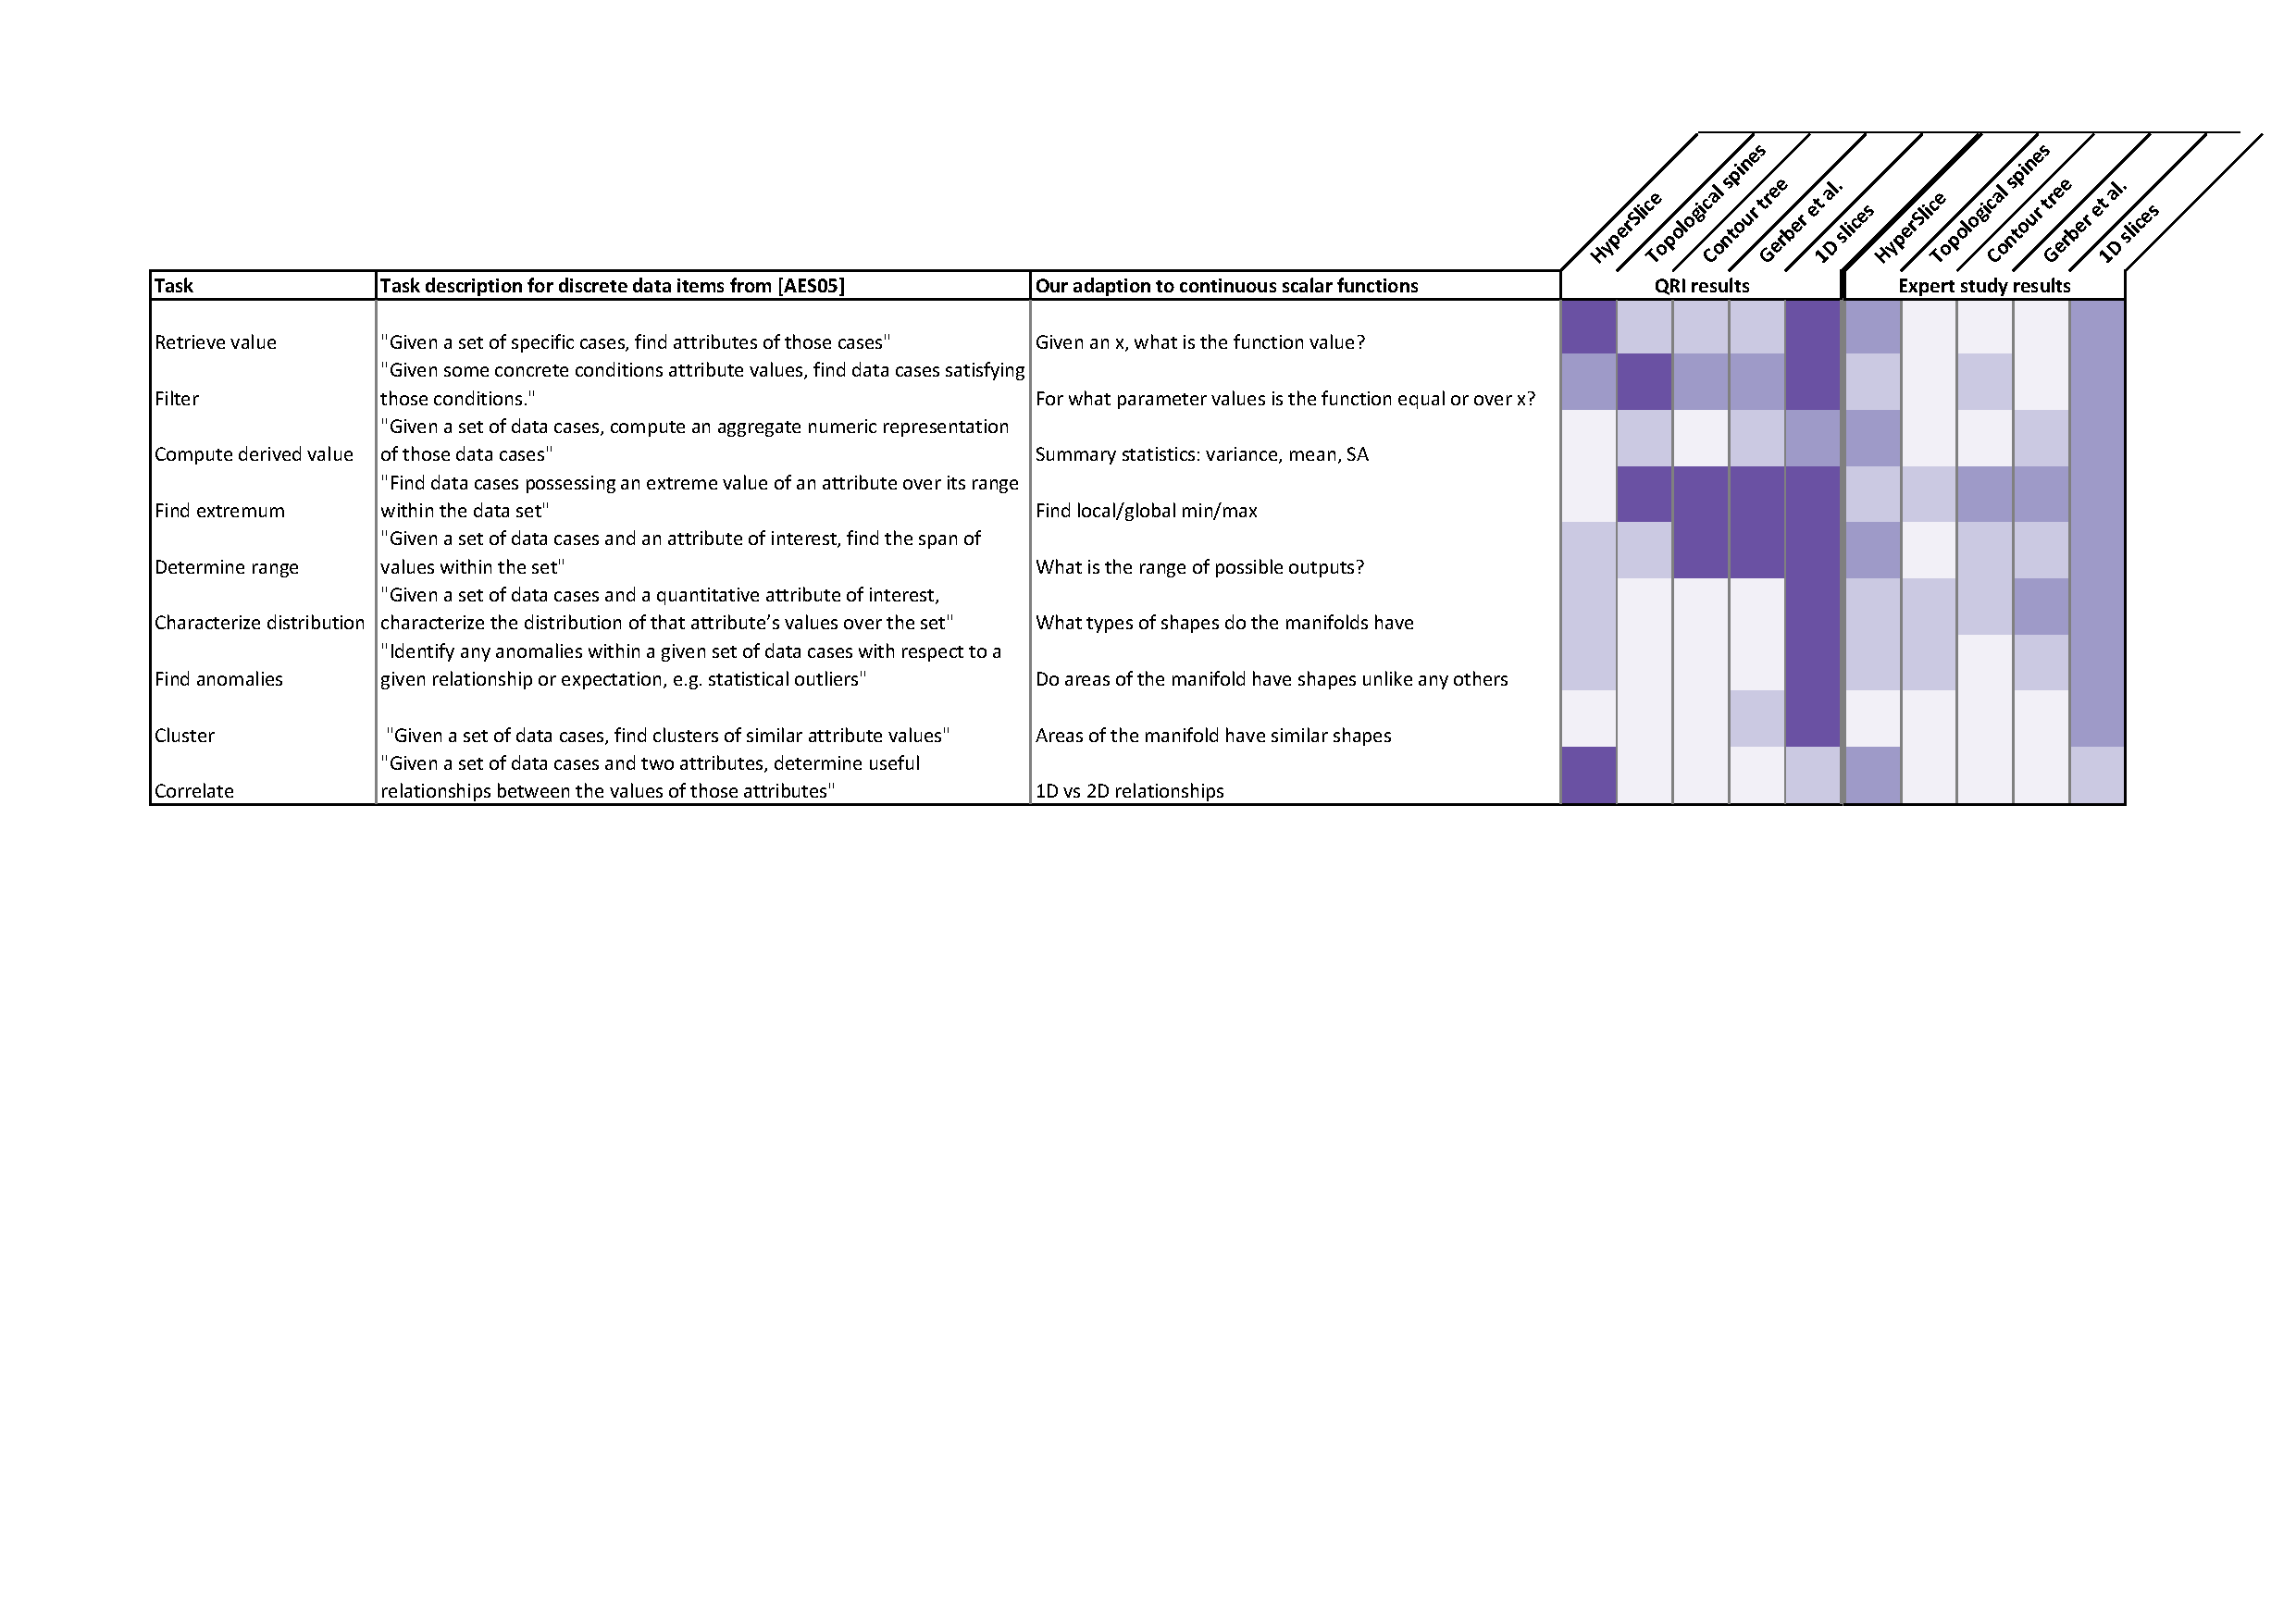
\includegraphics[width=\textwidth]{sp_task_list.pdf}
\end{table*}

\begin{figure}[tb]
  \centering
  \subcaptionbox{HyperSlice~\cite{Wijk:1993}\label{fig:compare:hs}}
    [0.48\textwidth]
    {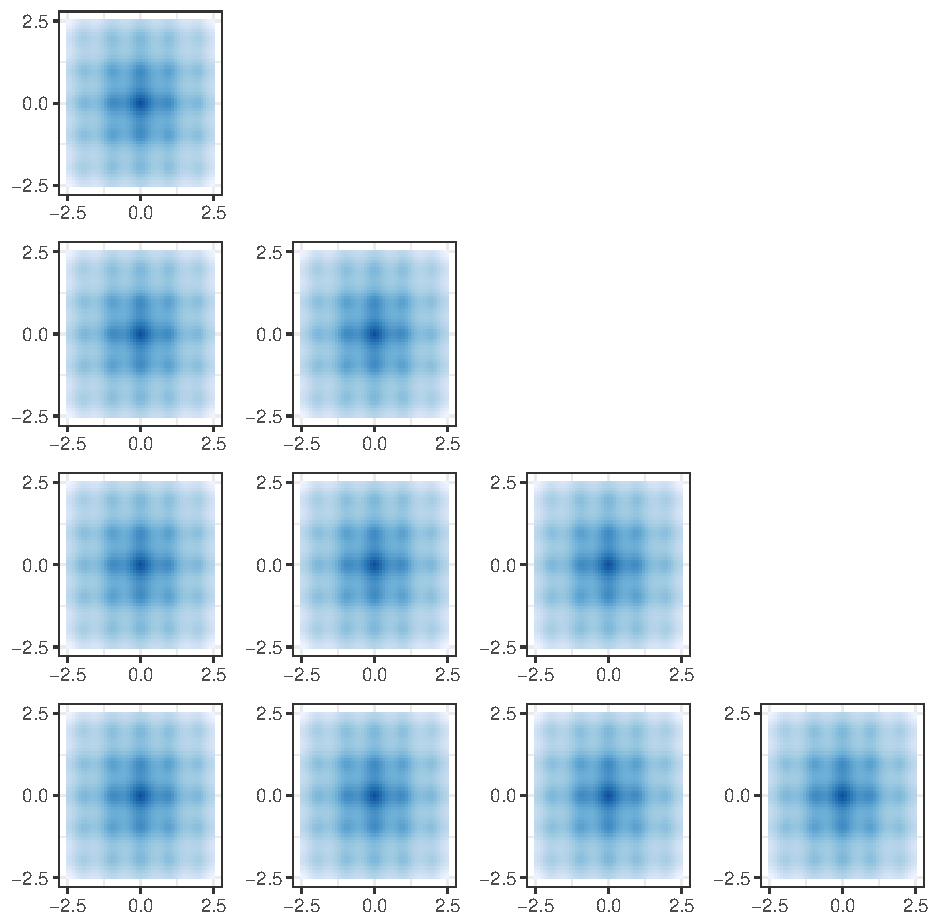
\includegraphics[width=0.17\textwidth]{ackley_5d_hs.pdf}}
  \hfill
  \subcaptionbox{Topological spine~\cite{Correa:2011}\label{fig:compare:ts}}
    [0.48\textwidth]
    {
\includegraphics[width=0.17\textwidth]{topo_spine.pdf}}
  \\
  \subcaptionbox{Contour tree~\cite{Carr:2003}\label{fig:compare:ct}}
    [0.48\textwidth]
    {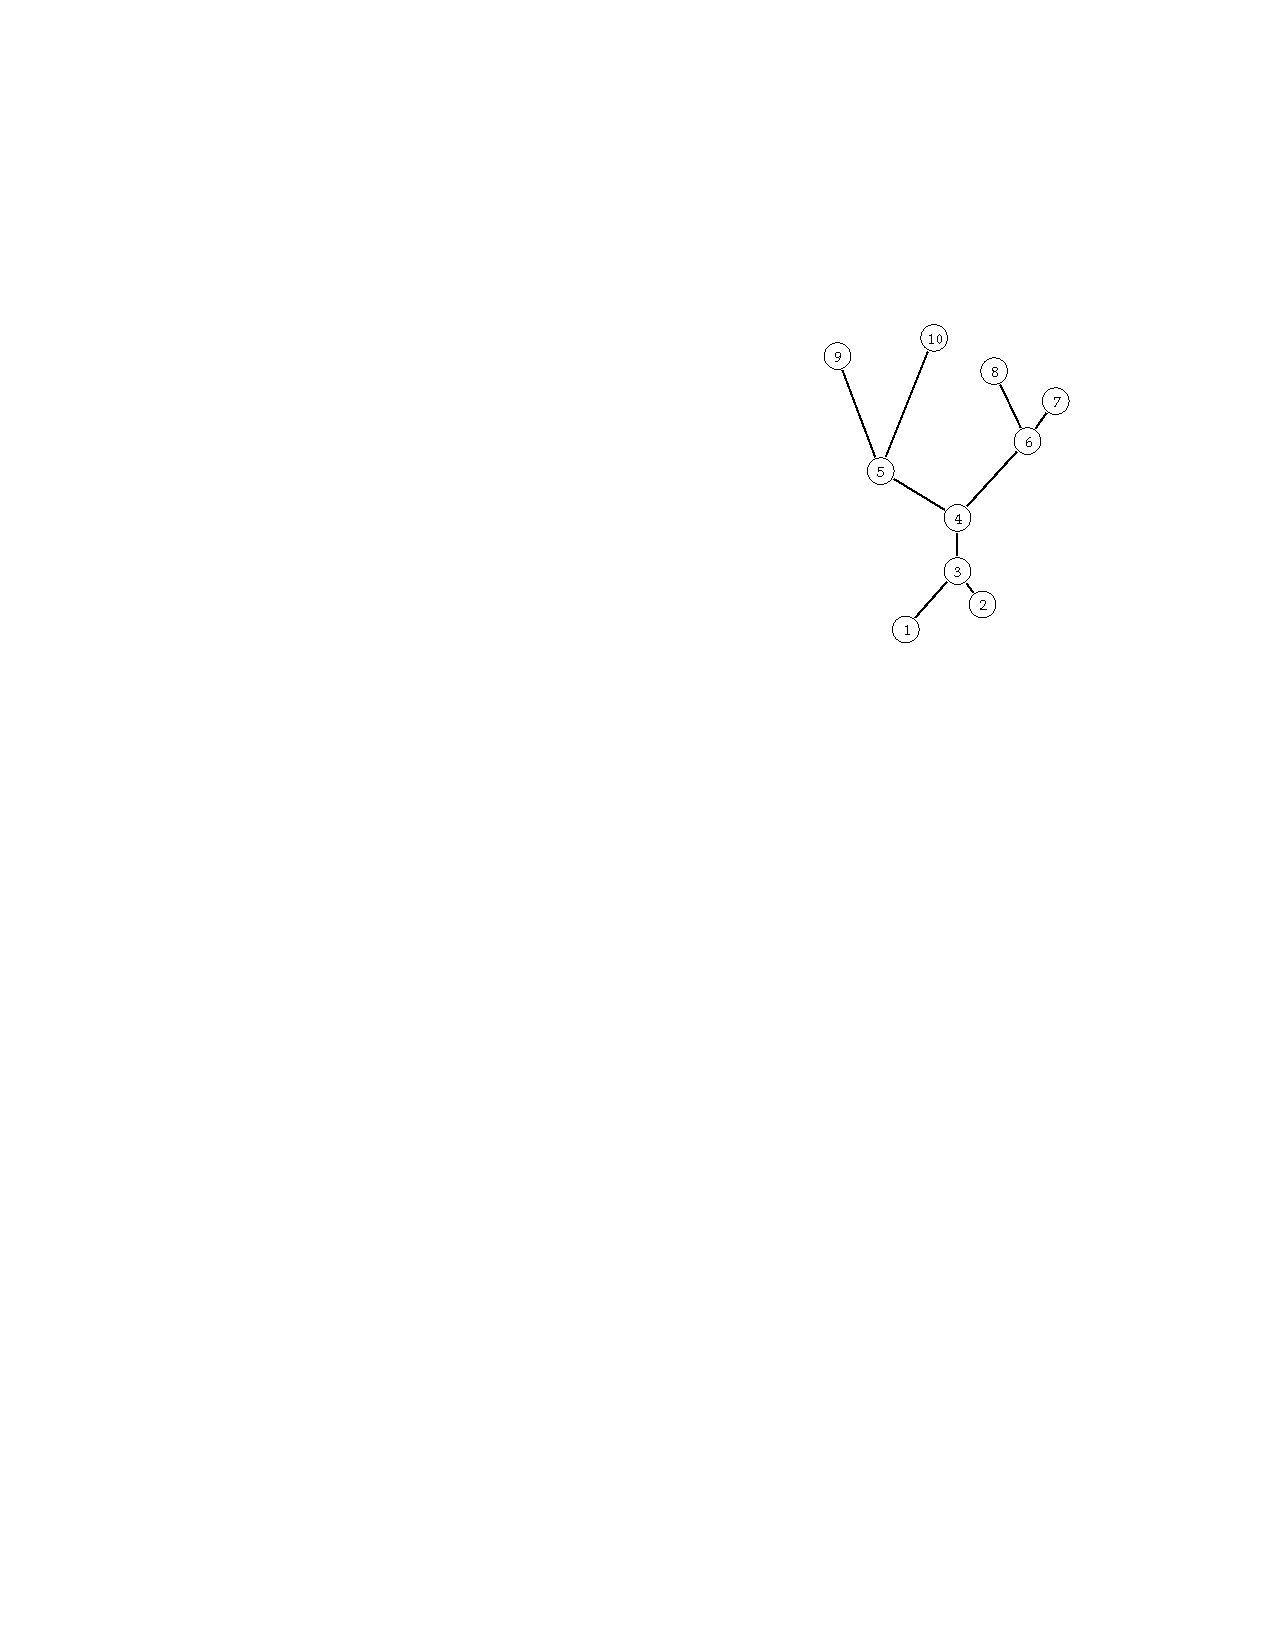
\includegraphics[width=0.17\textwidth]{contour_tree.pdf}}
  \hfill
  \subcaptionbox{Gerber et al.~\cite{Gerber:2010}\label{fig:compare:gerber}}
    [0.48\textwidth]
    {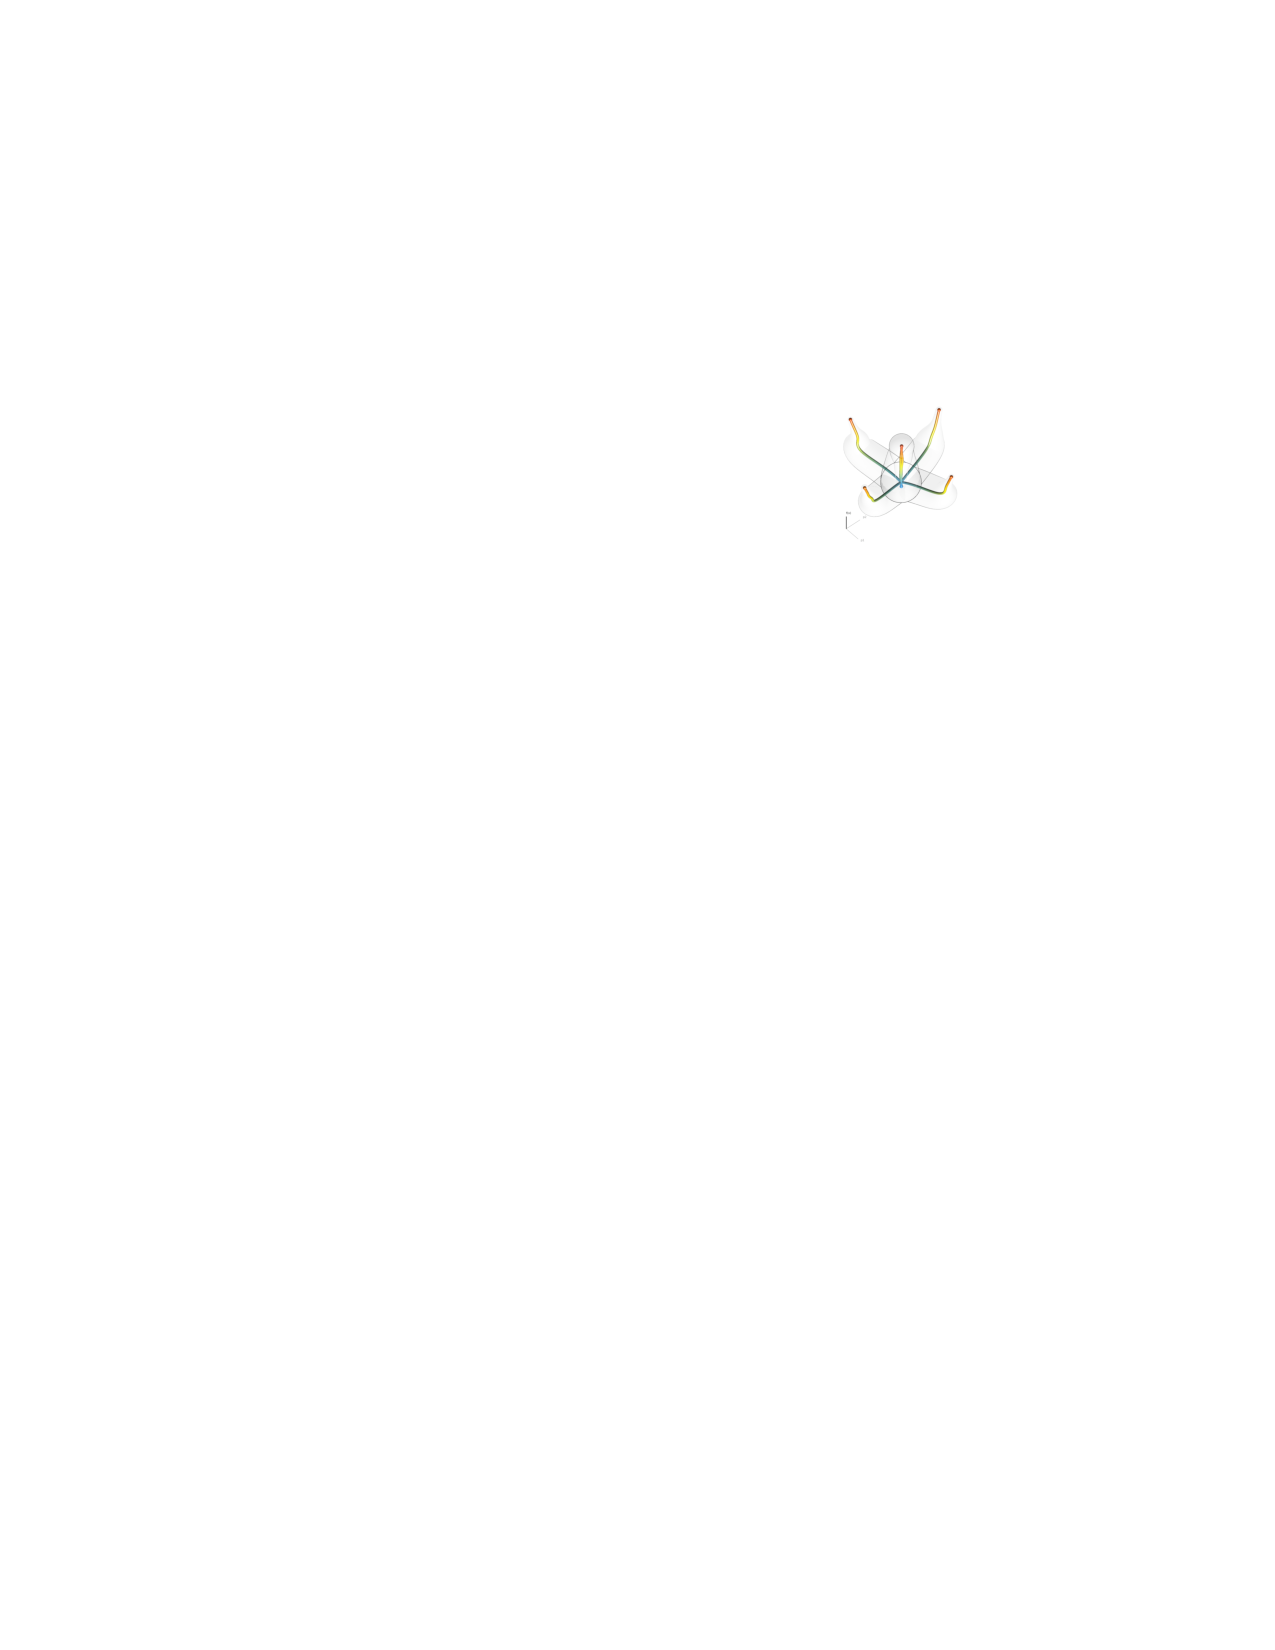
\includegraphics[width=0.17\textwidth]{gerber_ms.pdf}}
  %~
  %\subcaptionbox{1D slices\label{fig:compare:slices}}
    %[0.15\textwidth]
    %{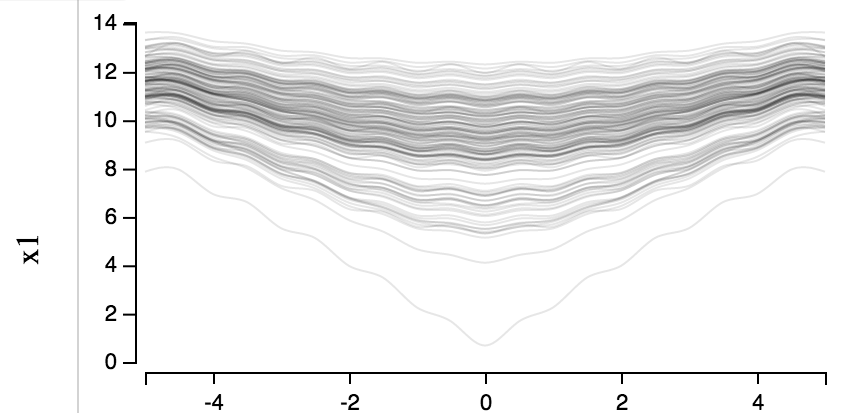
\includegraphics[width=0.1\textwidth]{images/4d_ackley_150slices.png}}
  \caption[The four techniques we used to compare with 1D slices.]{%
    The four techniques we used to compare with 1D slices. With
    the exception of HyperSlice, the images are from the respective papers and show different datasets used in their context.
  }
  \label{fig:compare}
\end{figure}

I first evaluate 1D slices in terms of their flexibility to deal with a broad
set of different low-level tasks.  Task taxonomies give a basis for comparing
visualization techniques to each other~\cite{Munzner:2014}.
If a technique addresses a large number of tasks, that is usually a good
indicator of its flexibility.  Over the last years, many different taxonomies
have been proposed~\cite{Amar:2005,Brehmer:2013,Heer:2012,Sedlmair:2014}.
However, to the best of my knowledge, none of these taxonomies thus far had a
dedicated focus on the visual analysis of multi-dimensional \textit{continuous}
data. I thus took a popular taxonomy for tasks on discrete data, by Amar,
Eagan, and Stasko~\cite{Amar:2005}, and extended each of their task categories
to directly address continuous data. This is an initial step towards
more consideration of multi-dimensional continuous data as a first class
citizen when developing task hierarchies.

Using this list of tasks, I compare 1D slices to other state of the art
techniques for multi-dimensional continuous data: HyperSlice~\cite{Wijk:1993},
topological spines~\cite{Correa:2011}, contour trees~\cite{Carr:2003}, and the
technique by Gerber et al.~\cite{Gerber:2010} (see \autoref{fig:compare}).  We
refer to topological spines, contour trees, and the work by Gerber et al.\ as
topological techniques when it makes sense to compare them as a group.
We evaluate based on all tasks, except for ``sort'', for which I could not
find a suitable extension to continuous functions.  The guiding theme in the
extensions is that users want to view the relationship of independent variables
to the dependent variable and to see how the dependent variable changes with
respect to the independent values.  The extensions are shown in
\autoref{tbl:task_list} along with the results of two investigations we
conducted based on them, as detailed in the following section.
\subsection{Study design}

To perform a task-based evaluation, I investigated the different techniques in two different ways.
First, I used a \textit{qualitative result inspection}
approach~\cite{Isenberg:2013}. 
I iteratively analyzed the techniques with different datasets and summarized
our discussion and analysis on a four point scale:
``None'' means that it is not possible to perform the task with the technique,
``partly'' means that it requires major interaction with the view to accomplish
the task, ``mostly'' means that one can accomplish the task with little
interaction, and ``fully'' means that this task is directly addressed by the
technique. 

Second, in order to get a more objective judgment I also asked 
\textit{four visualization experts} familiar with examining multi-dimensional spaces like
parameter space exploration to examine the eight datasets with different
techniques and rate how well each task can be accomplished with each technique
on the same scale. \autoref{fig:compare} shows the averaged results along with the
results of the qualitative result inspection in \autoref{fig:compare}.

For the techniques, I use my own implementation of HyperSlice and topological
spines since no code was available. I used the \texttt{msr} R
package~\cite{Gerber:2012} which implements the algorithm of Gerber et
al.~\cite{Gerber:2010}. For the contour tree I used the \texttt{libtourtre}
library and then rendered the trees using GraphViz using the
Sugiyama~\cite{Gansner:1993} layout.  As datasets, I chose the 2D sinc
function, 5D Rosenbrock~\cite{Rosenbrock:1960} function, 6D Ackley function, a
26 node hidden layer neural network built on the Boston housing
dataset~\cite{Lichman:2013}, a support vector machine with Gaussian kernel
built on the housing dataset, the fuel 3D volume dataset~\cite{Roettger:2017},
and the neghip 3D volume dataset~\cite{Roettger:2017}.  
Not all datasets could be rendered with all techniques due to software errors.

\subsection{Results}\label{sec:task-solutions}

In this section, I summarize our discussion about the strengths and weaknesses
of each technique in terms of performing the task.  For more details, there is
also a website that contains details of how each visualization technique can
solve each task. The website is available at
\url{http://sliceplorer.cs.univie.ac.at}.

%\msnote{TO-DISCUSS why is extending tasks from discrete to continuous domain a valid approach?}

\textbf{Retrieve value}:\label{retrieve-value}
In the discrete case, the user should be able to look at a point and get the
detailed values of it. In the continuous case we are interested in what the
function value is for a certain input parameter setting. All the techniques
support this although with the topological methods this is only possible for
the extrema and saddle points as all other points are filtered out. For
example, there could be many points between node $4$ and $5$ in the contour
tree (\autoref{fig:compare:ct}). With
slicing techniques, both 1D and 2D, the values can be read directly off the
chart. Of course, for all techniques the adding of interaction, such as a tooltip, can make retrieving concrete values even easier. 

\textbf{Filter}:\label{filter}
Amar, Eagan, and Stasko describe this task as a general filtering query on data points.
In the continuous case, the user wants to understand the outputs of the
function. This is a query as to where the function value is in a certain range.
With continuous data this is the domain of isosurface extraction.
This is possible with slicing techniques by visual examination.
With HyperSlice, though, one must be careful to view sufficient focus points to
get a general idea of where the function equals certain values.  Topological
spines also shows this directly and they use concentric areas 
(\autoref{fig:compare:ts}) to give a
general idea of the area that a particular value range takes up. The other
topological techniques allow one to see if a certain value is possible, for
example, we can see that the function represented by the contour tree in 
\autoref{fig:compare:ct} takes the values greater than 4 somewhere by seeing 
that there are edges from node 4 to nodes 5 and 6. However,
there is no relation back to the parameter settings that will produce these
values. 

\textbf{Compute derived value}:\label{compute-derived-value}
The direct interpretation of this task to continuous data is to compute derived
value results about the curves 
%\msnote{TO-DISCUSS: the curves? all 1D ones for one dimension? What about derived values that summarize the entire function?} 
like mean and variance. Many of these values can
also be perceived visually.  Topological methods compute the persistence value
between the function to determine what to show but with the exception of
topological spines this is hidden from the user. Topoplogical spines show a
graph of the persistence and ``saturated persistence'' which allows the user
to select which nodes to filter.
Projections of 1D curves allows us to see the distribution.
In
\autoref{fig:walkthrough}c we can see that there are very few function values
around the global minimum and the function has two types of behavior: a
periodic sine wave across the domain and a general parabola shape.

\textbf{Find extremum}:\label{find-extremum}
All the topological techniques we evaluated support this in some
way. With HyperSlice one needs substantial guidance on setting the focus point to find
extrema (like a histogram of function outputs). % or a gradient widget.  Since
1D slices is a global technique showing all slices at once, one can find
extrema by inspecting the graphs.
% see this
%directly since the slices are projected. Extreme values can be seen visually.
As previously mentioned, topological methods are purpose built to extract
extrema from continuous data. For example, it is easy to see that the function
using the method by Gerber et al.\ (\autoref{fig:compare:gerber}) has five
maxima and the function of the contour tree (\autoref{fig:compare:ct}) has four
maxima.

\textbf{Determine range}:\label{determine-range}
Amar, Eagan, and Stasko describe this as finding the range of possible values
for a particular attribute. There is really only one attribute of interest: the
values of the multi-dimensional scalar function. Any view from which we can
read the global minimum or the global maximum allows us to do this. Contour
trees, Gerber et al., and 1D slices all allow us to read these off the view.
Topological spines either show the global maximum \emph{or} the global minimum,
but not both.  HyperSlice has no way to do this directly by adjusting the focus
point.  However, one expert noticed that they could simply read the range of
the function off of the color legend.

\textbf{Characterize Distribution}:
\label{characterize-distribution}
Here again there is one key value of interest that we want to characterize: the
function value.  This requires a global view.  Projections of slices directly
show how the function slices are distributed.  We can see in
\autoref{fig:walkthrough}d that there are very few function values around the
global minimum but many around high values. It would be difficult to use
HyperSlice to truly understand the distribution of values. The user would
somehow have to browse around the focus points and then memorize the function
values. Topology throws away the spatial element and just shows the
relationships between extrema and saddles.

\textbf{Find anomalies}:\label{find-anomalies}
%\msnote{TO-DISCUSS what does an outlier mean in continuous lands? Is it really about shapes? Or is it about spiky-ish behavior?}
Anomalies in the discrete case are single point outliers. While that is also
possible in the continuous case, we may also have entire parts of the function
that are unlike any other part. These should also be identified.
In a global view like projected 1D slices these will show up visually. The
slices will stand out from the rest similar to other projection-based
techniques like scatterplots. With HyperSlice we must browse around until we
can see one directly. However, we will see it if we can find it. Topological
methods will only show extrema in terms of maxima or minima values but not
shape and hence mask anomalies and outliers.

\textbf{Cluster}:\label{cluster}
Since we are looking at manifold behaviors, we want to be able to group the
functions into areas of similar behavior. For example, are they monotonically
increasing or decreasing? Furthermore, can we find areas where the variance
changes? The topological technique of Gerber et al.~\cite{Gerber:2010} was
created to address just this. They split the function
into areas of monotonic behavior and then show a line indicating how those
monotonic regions are related to each other. However, the way they
reconstruct the function between extrema and saddle points does not allow us to
view the variance between these points as the 1D slice view
allows. Clustering the 1D slices tries to split the slices into groups of
similar behavior (see \autoref{fig:cluster:clustered}).

%\begin{figure}
  %\centering
  %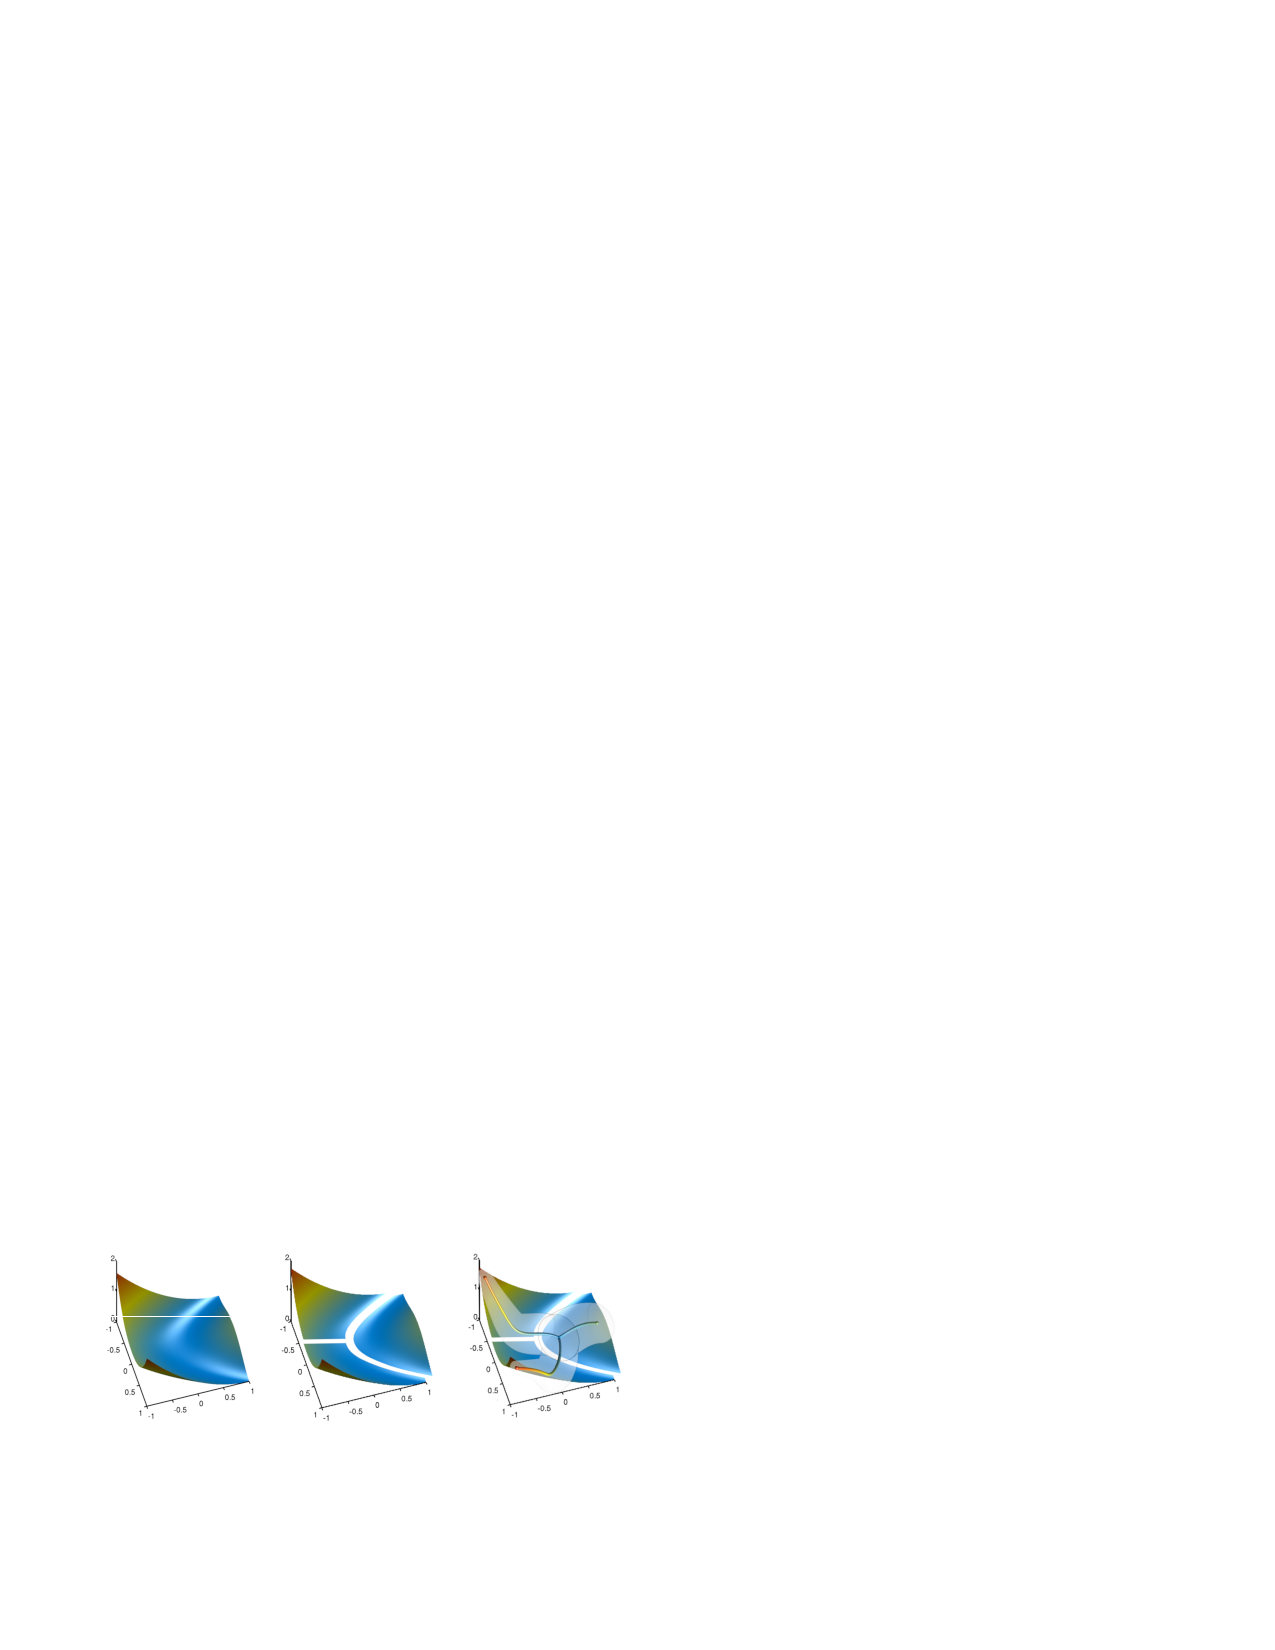
\includegraphics[width=\columnwidth]{images/gerber_evolution.pdf}
  %\caption{
    %How the method of Gerber et al.\ visualizes a function. They take a 
    %function (left image), decompose it into areas of monotonic behavior 
    %(center image), approximate each region with a regression model (right
    %image), and then show this regression model to the user.
    %(image from \cite{Gerber:2010}).
  %}
  %\label{fig:gerber}
%\end{figure}

\textbf{Correlate}:\label{correlate}
Finally, we consider correlation. In the discrete data case the goal is to find
correlation between attributes. With continuous data, we already have a
dependency between the independent and dependent variables. What we would like
to learn is how many variables have an influence on the function. With 2D views
(that only HyperSlice provides) one can see both 1D and 2D interactions with
the function. We can see that the function in \autoref{fig:compare:hs} has
radial behavior so the function value depends on both 1D and 2D interactions.
None of the other techniques are capable of showing 2D interactions between
parameters.

\subsection{Summary}

From the summary in \autoref{tbl:task_list} we can see that the 1D slices
technique addresses more of the tasks than any other technique.  It is not
always the highest performing view though.  HyperSlice is the only technique 
evaluated that could show more than one-dimensional interactions but it does
not do well on global tasks like extrema detection. The various topological
techniques directly address tasks related to extrema detection and comparison
but do not perform as well on others. 
%\ttwnote{should the following go in limitations?}
The experts often commented that they felt they needed more knowledge about
what exactly the topological techniques were doing in order to interpret
the results. Thus, the ratings for these techniques may be artificially low.
%\ttwnote{However, given the difficulty that experts had with the technique,
%this does not bode well for the general public.}
I conclude that 1D slices are a
very flexible technique indeed.  



\section{Usage scenarios}\label{sec:usage-scenarios}

In addition to evaluating 1D slices with a low-level task hierarchy, we also
provide usage scenarios to understand their value in real-world applications.
We begin with an illustrative example using the 2D sinc
function.
%\ttwnote{cite?}.  TM: No need to cite!
We then use our 1D slices approach to illustrate how
it can help better understand neural network architectures for a regression
problem. Finally, we use 1D slices to investigate the effect of initial
position on optimization algorithm performance.

The purpose of these evaluations is a proof of concept that 1D slices can be
used for real-world problems. In particular, it is not meant as a comparative
evaluation as provided in the previous section. To the best of our knowledge,
neither HyperSlices nor topological techniques have been applied to
understanding neural networks nor optimization algorithms so far. A full
adaption of, and comparison to, these techniques for the provided use cases are
beyond the scope of this paper, and are left for future work. 

\subsection{2D sinc function}

\begin{figure}
  \centering
  \begin{subfigure}[b]{0.3\linewidth}
    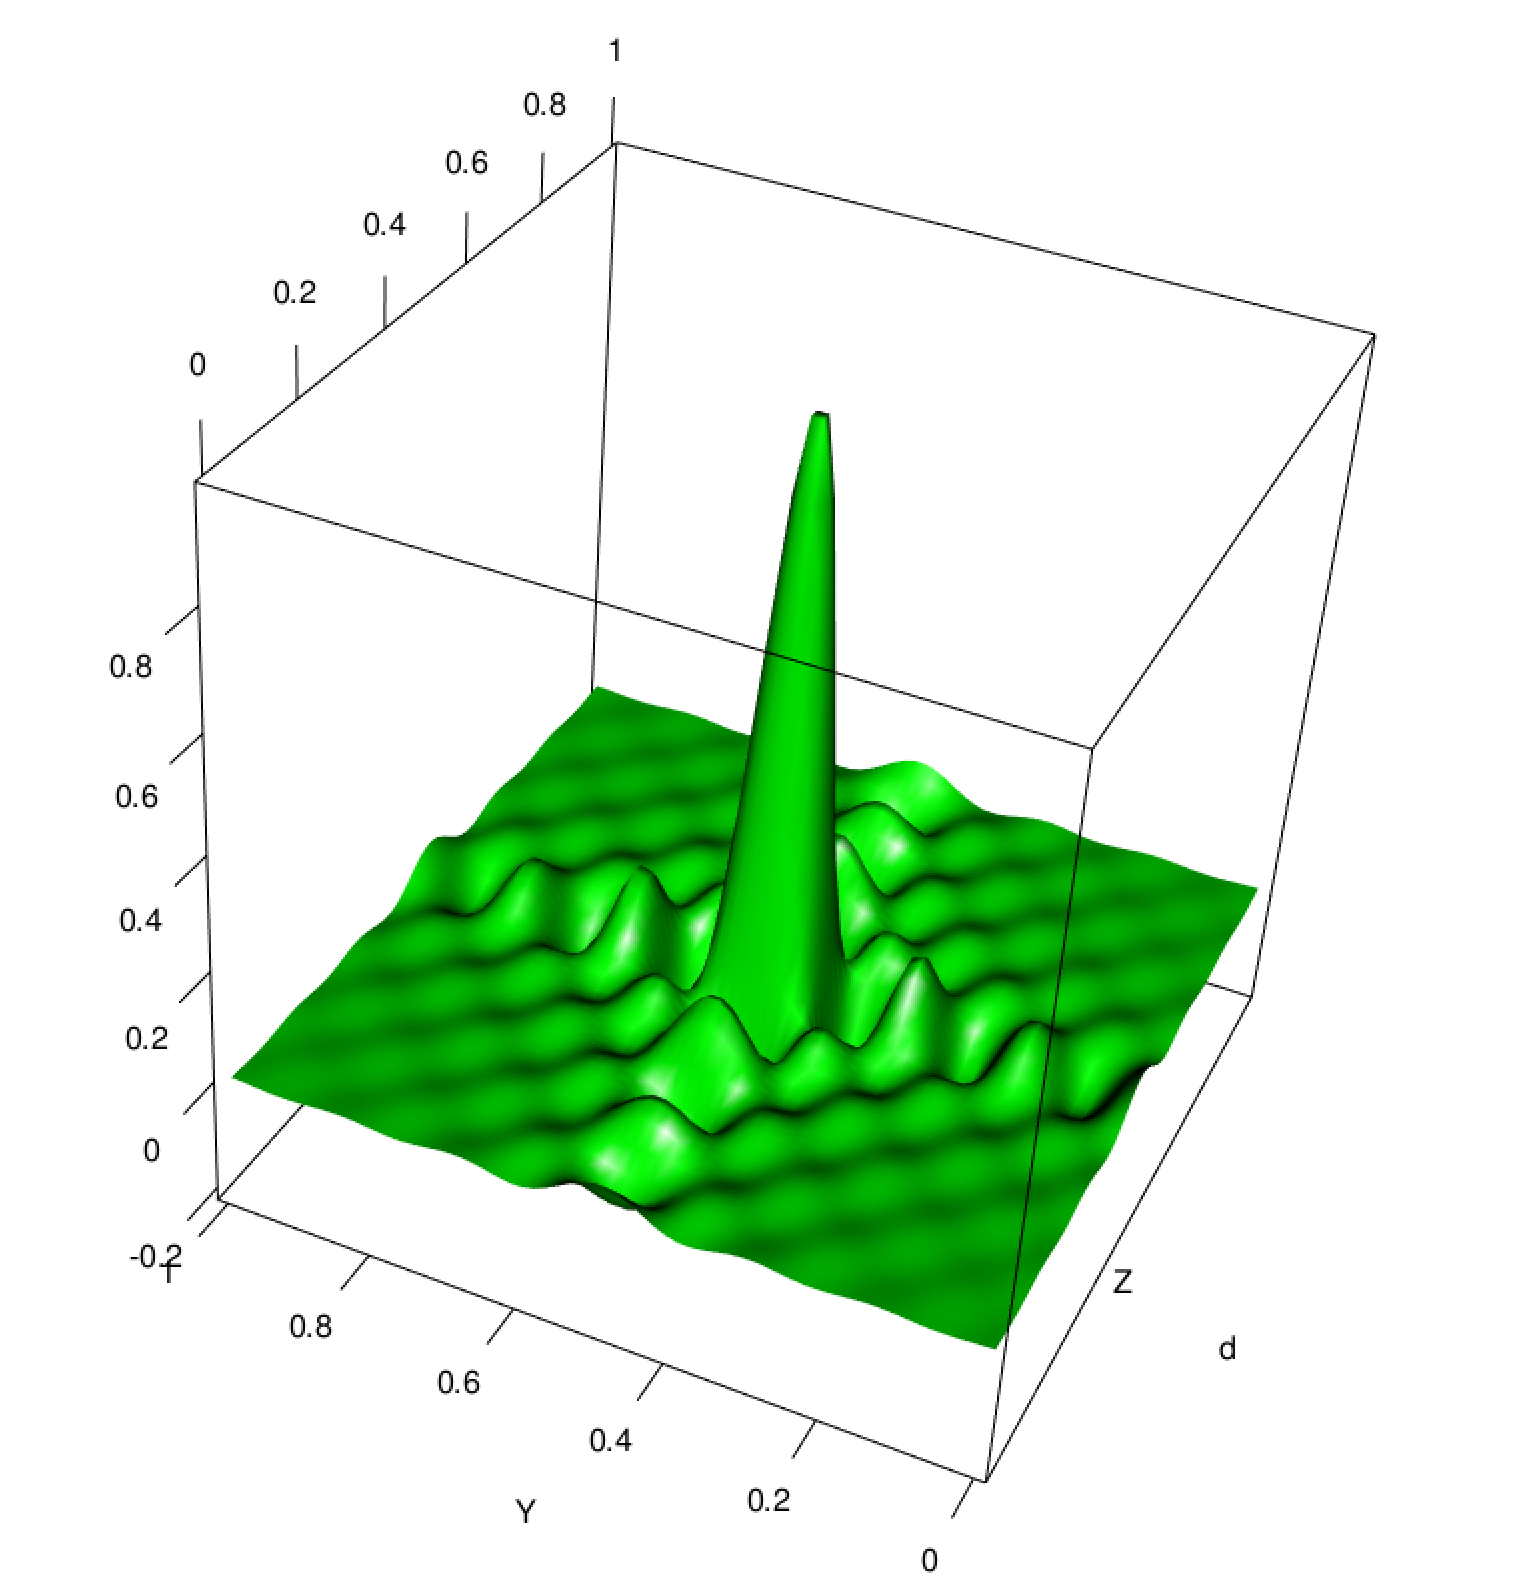
\includegraphics[width=\textwidth]{sinc_3d.png}
    \caption{
      Surface plot
    }
    \label{fig:sinc:3d}
  \end{subfigure}
  \qquad\qquad%
  \begin{subfigure}[b]{0.3\linewidth}
    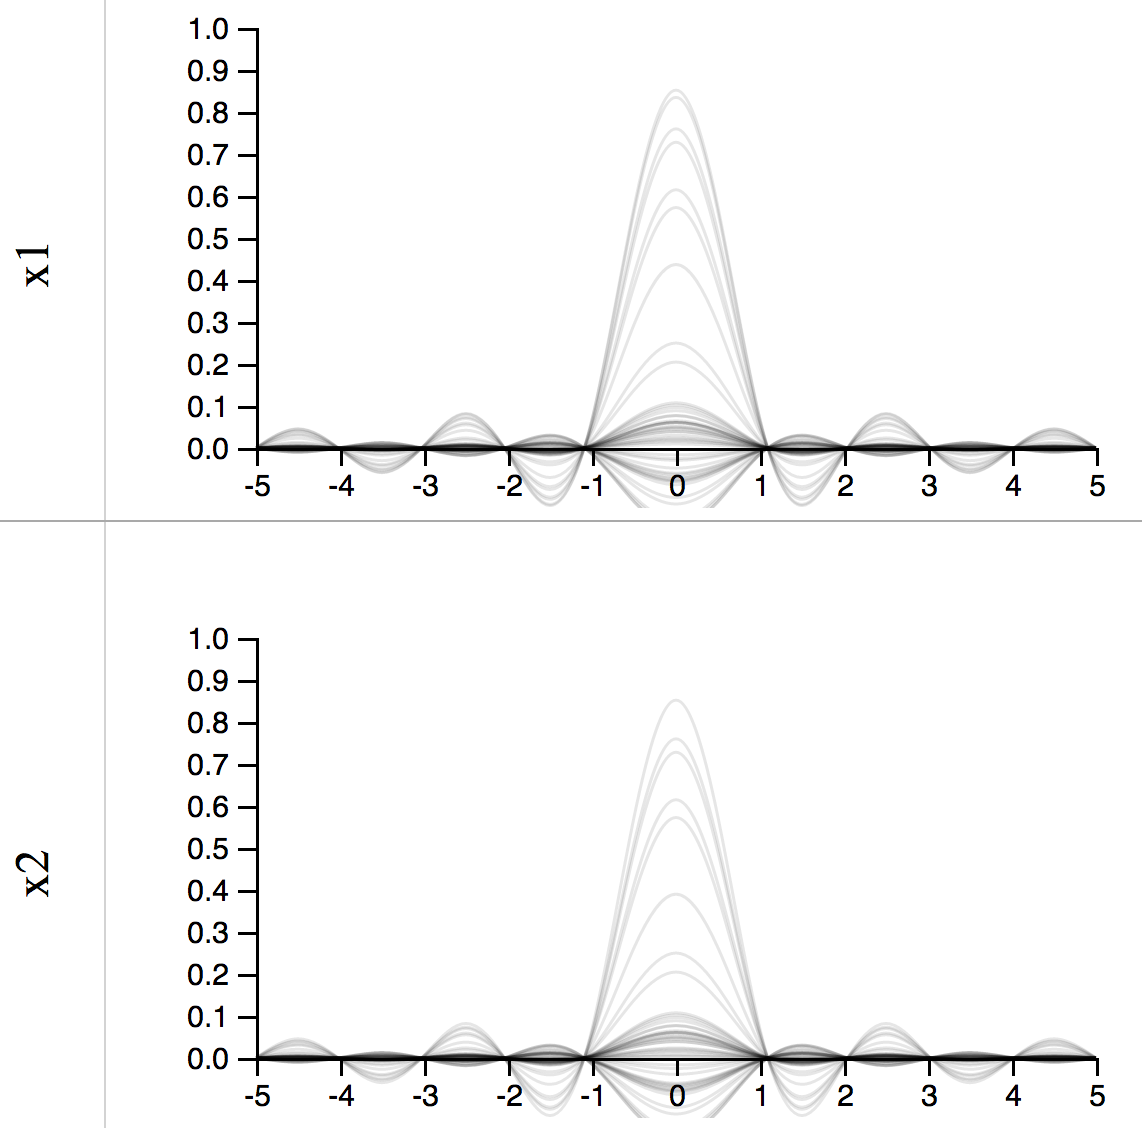
\includegraphics[width=\textwidth]{sinc_sp.png}
    \caption{
      1D slices
    }
    \label{fig:sinc:sp}
  \end{subfigure}
  \\
  \begin{subfigure}[b]{0.3\linewidth}
    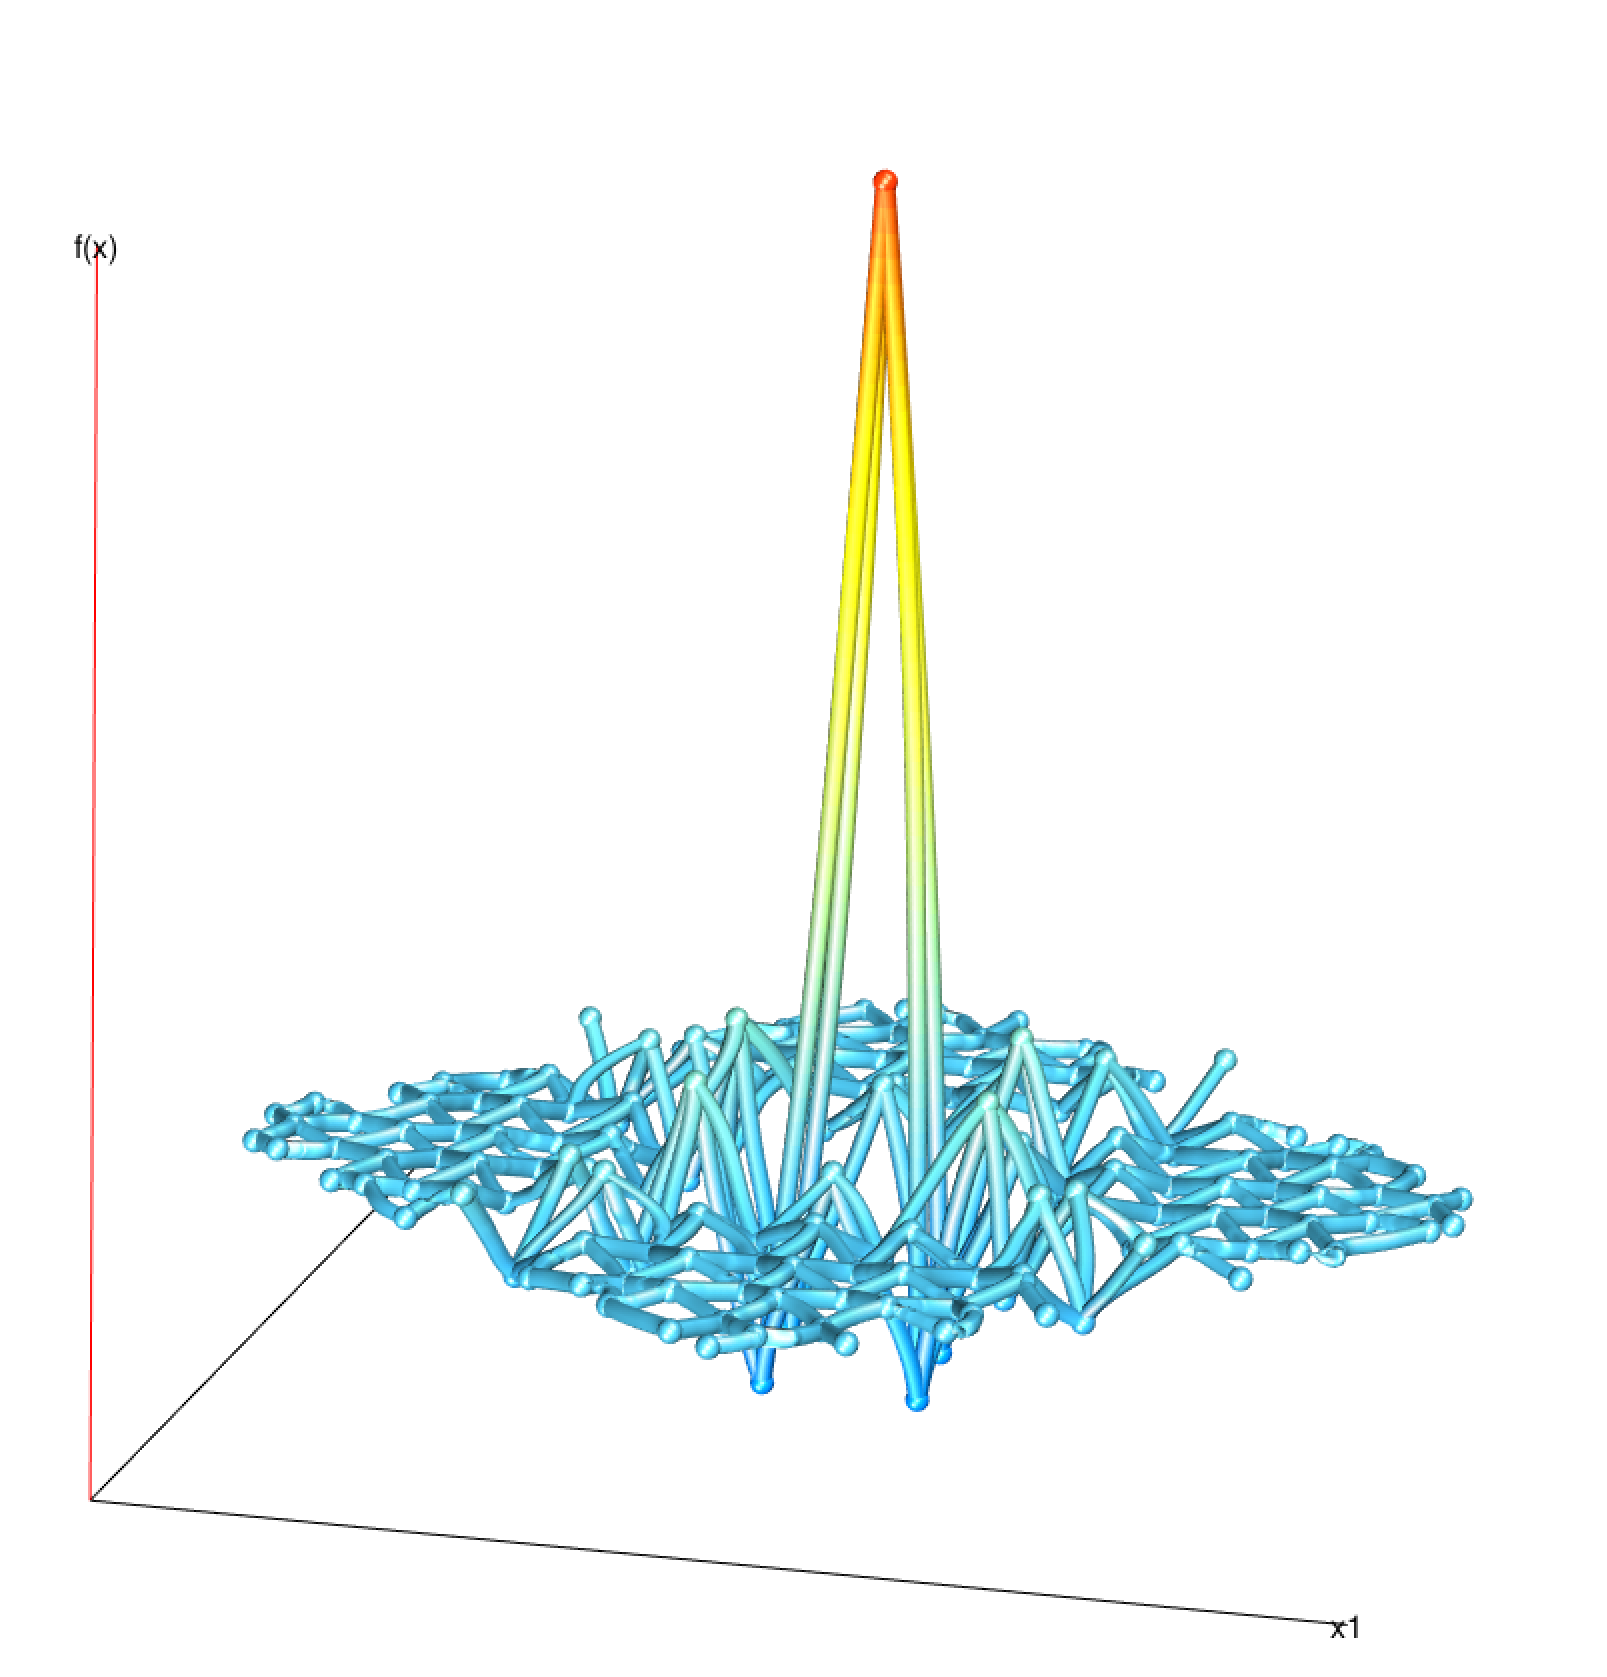
\includegraphics[width=\textwidth]{sinc_ms_1.png}
    \caption{
      $\texttt{pLevel} = 0.0$
    }
    \label{fig:sinc:ms_1}
  \end{subfigure}
  \hfill
  \begin{subfigure}[b]{0.3\linewidth}
    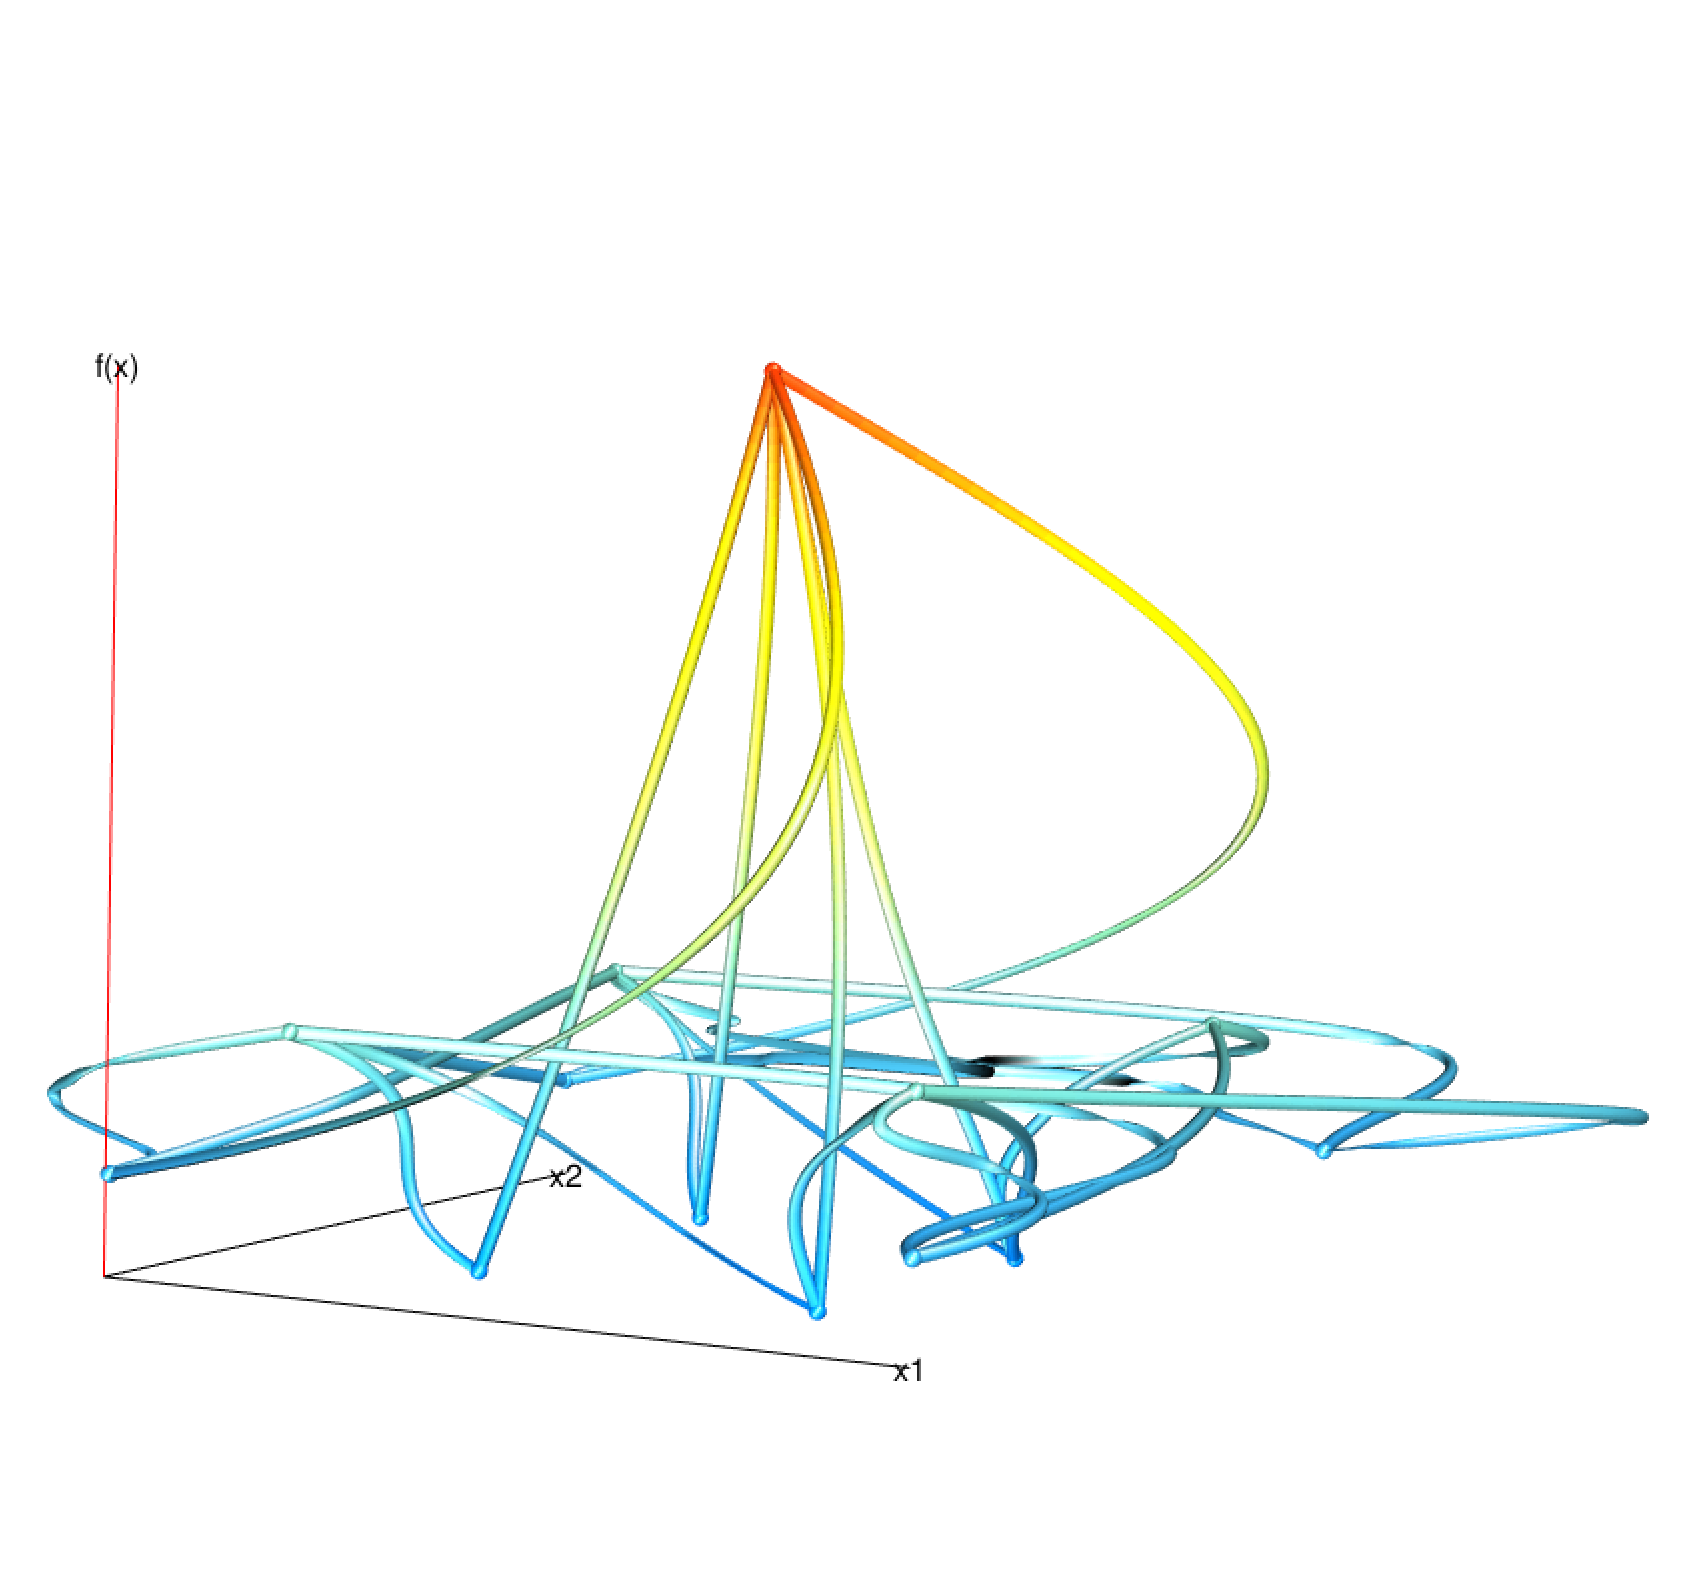
\includegraphics[width=\textwidth]{sinc_ms_2.png}
    \caption{
      $\texttt{pLevel} = 0.05$
    }
    \label{fig:sinc:ms_2}
  \end{subfigure}
  \hfill
  \begin{subfigure}[b]{0.3\linewidth}
    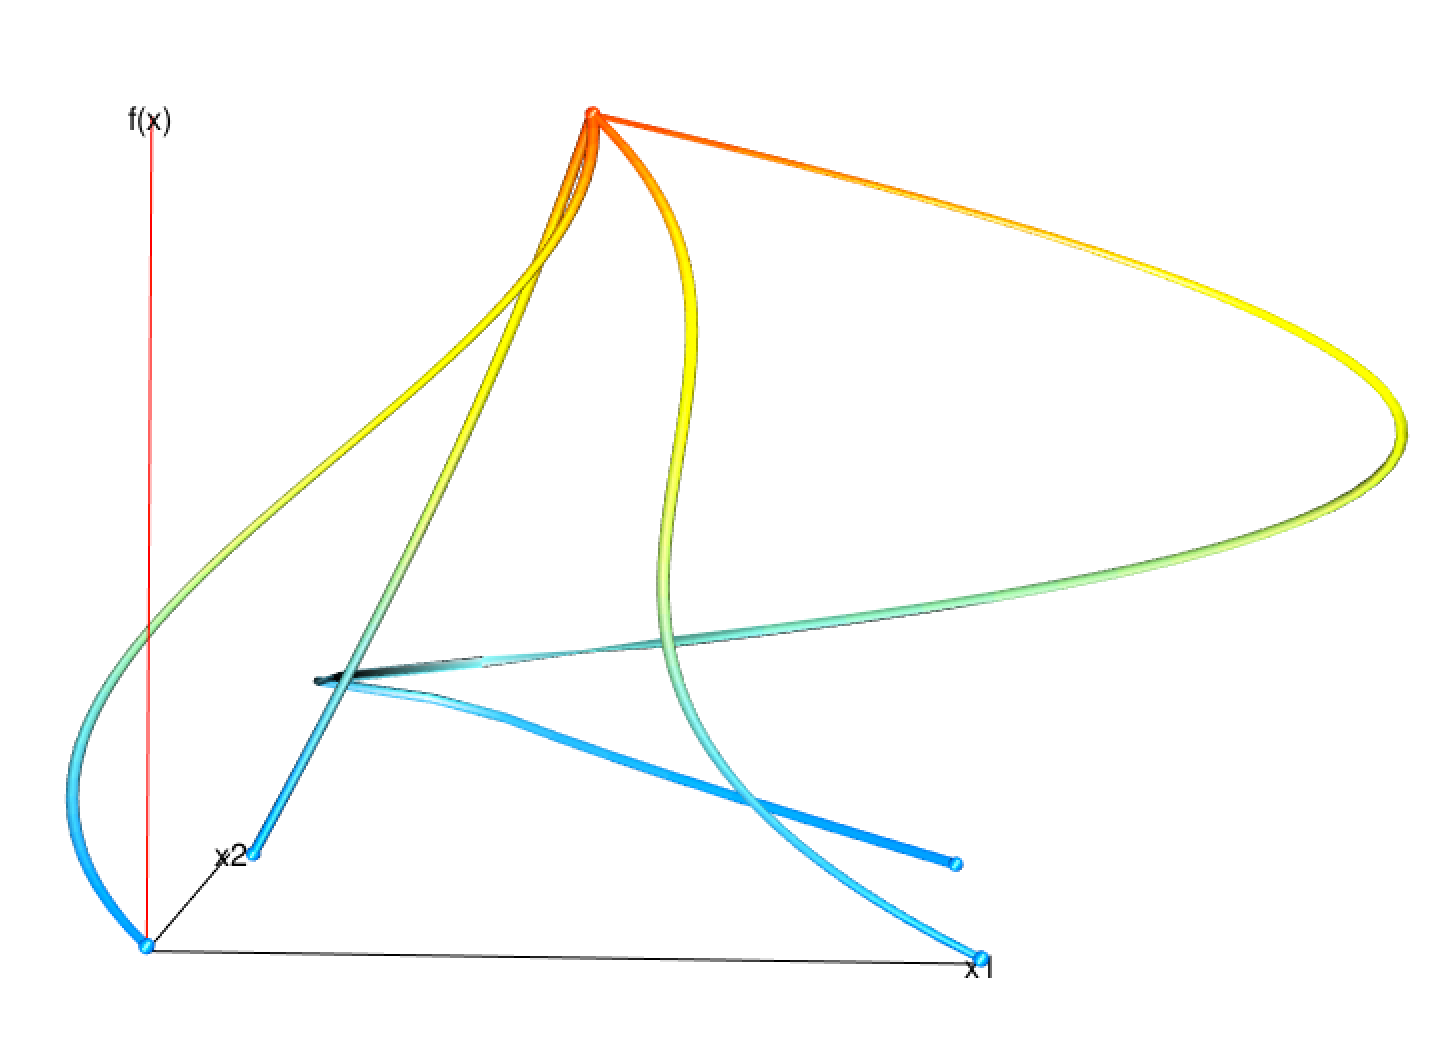
\includegraphics[width=\textwidth]{sinc_ms_3.png}
    \caption{
      $\texttt{pLevel} = 0.1$
    }
    \label{fig:sinc:ms_3}
  \end{subfigure}
  \caption{
    Different views of the 2D sinc function. We show the surface plot
    in (\subref{fig:sinc:3d}) for reference. Our 1D slice view is shown
    in (\subref{fig:sinc:sp}). The central peak as well as the sub peaks
    are prominent. For comparison we show the method of Gerber et 
    al.~\cite{Gerber:2010} in 
    (\subref{fig:sinc:ms_1})--(\subref{fig:sinc:ms_3}) at different levels 
    of persistence filtering. 
    With no filtering (\subref{fig:sinc:ms_1}) the graph looks much like the
    original function. The plot is very sensitive to the filtering level.
    (\subref{fig:sinc:ms_2}) and (\subref{fig:sinc:ms_3}) are all very 
    different from each other.
  }
  \label{fig:sinc}
\end{figure}

Imagining how a function in more than 3-dimensions looks is difficult if not
impossible. In order to illustrate how Sliceplorer visualizes functions we show
the 2D sinc function. 
%\tmnote{The sinc function is a the perfect reconstruction function in the band limited case.}
We are using the formulation where 
$y(x_1,x_2) = \frac{sin(\pi x_1)}{\pi x_1} \frac{sin(\pi x_2)}{\pi x_2}$.
In \autoref{fig:sinc:3d} we show a 3D surface plot of this function. The 
global maximum is at $x_1,x_2 = 0,0$ where $y=1$. There are a number of local
maxima and minima of decreasing value radiating out from the origin.

We show the 1D slice view using Sliceplorer in \autoref{fig:sinc:sp}.
We are showing 50 slices in each of the 2 plots. We can clearly see that
the maximum value occurs when $x_1,x_2 = 0,0$ in the graph at around $y=1$.
We can also see the decreasing extrema radiating out from the origin. We can
also precisely measure the height and x-location of the extrema. If we want
to examine a particular trace then we can highlight it in the view and see
the full slice highlighted on screen.

For comparison, we show visualizations of the 2D sinc function rendered using
the \texttt{msr} package~\cite{Gerber:2012} in R. This package implements the
visualization of the Morse-Smale complex from Gerber et al.~\cite{Gerber:2010}.
We sampled the function with $2000$ sample points using a Sobol sequence. The
1D slices view is showing $50$ focus points with $21$ samples for each slice so
this was done to use a similar sampling method and number of samples to the
Sliceplorer method. The function can do persistence-based filtering of the
graph before rendering.  This is controlled by the \texttt{pLevel} parameter
which filters all persistences less than a certain value. In
\autoref{fig:sinc:ms_1} we show the view with the filtering level set to $0$,
i.e.\ no filtering. The view does a very good job showing the critical points
of the graph. It looks very similar to the surface plot
(\autoref{fig:sinc:3d}). However, the visualization is very sensitive to the
filtering level. In \autoref{fig:sinc:ms_2} and \autoref{fig:sinc:ms_3} we show
the sinc function with the filtering level set to $0.05$ and $0.1$
respectively.  The 1D slice view does not suffer from this issue of
parameterization.

\subsection{Neural networks}\label{neural-networks}

\begin{figure*}[t]
  \centering
  \begin{tabular}[b]{cccc}
    Neural network - 26 & SVM - polynomial & Neural network 5+3 & SVM - radial \\
    \hline \\
    \begin{subfigure}[b]{0.2\textwidth}
      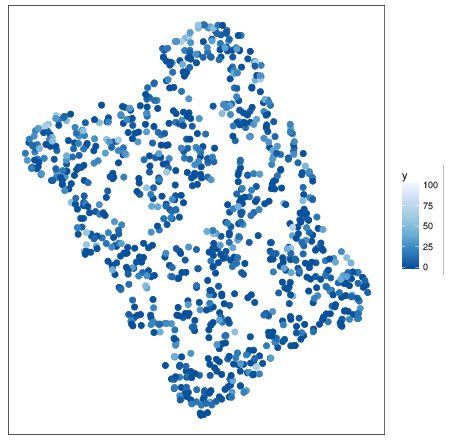
\includegraphics[width=\textwidth]{boston_nn_26_sp.png}
      \caption{
      }
      \label{fig:nn_comp:a}
    \end{subfigure}
    &
    \begin{subfigure}[b]{0.2\textwidth}
      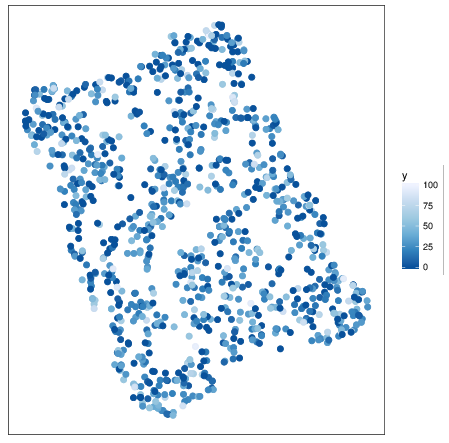
\includegraphics[width=\textwidth]{boston_svm_poly_sp.png}
      \caption{
      }
      \label{fig:nn_comp:b}
    \end{subfigure}
    &
    \begin{subfigure}[b]{0.2\textwidth}
      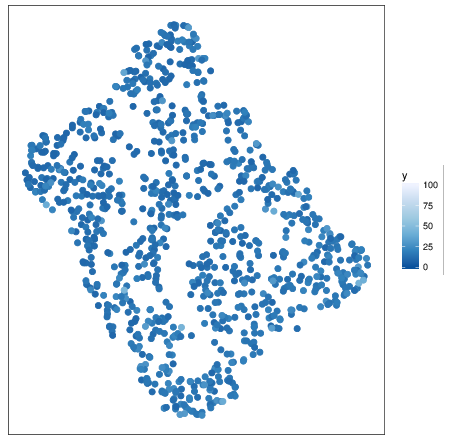
\includegraphics[width=\textwidth]{boston_nn_5x3_sp.png}
      \caption{
      }
      \label{fig:nn_comp:c}
    \end{subfigure}
    &
    \begin{subfigure}[b]{0.2\textwidth}
      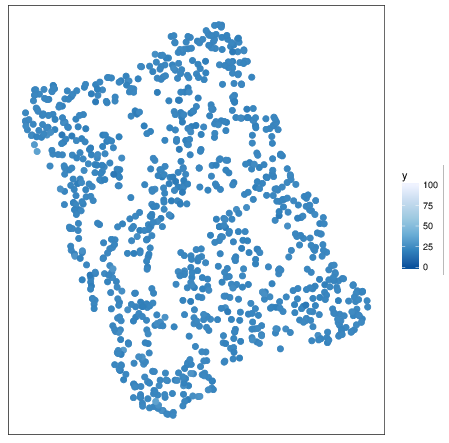
\includegraphics[width=\textwidth]{boston_svm_radial_sp.png}
      \caption{
      }
      \label{fig:nn_comp:d}
    \end{subfigure} \\
    \begin{subfigure}[b]{0.2\textwidth}
      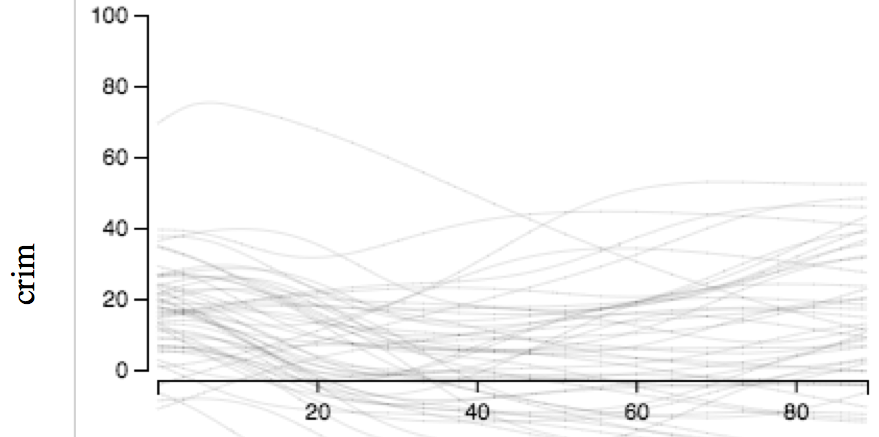
\includegraphics[width=\textwidth]{boston_nn_26_slices.png}
      \caption{
      }
      \label{fig:nn_slices:e}
    \end{subfigure}
    &
    \begin{subfigure}[b]{0.2\textwidth}
      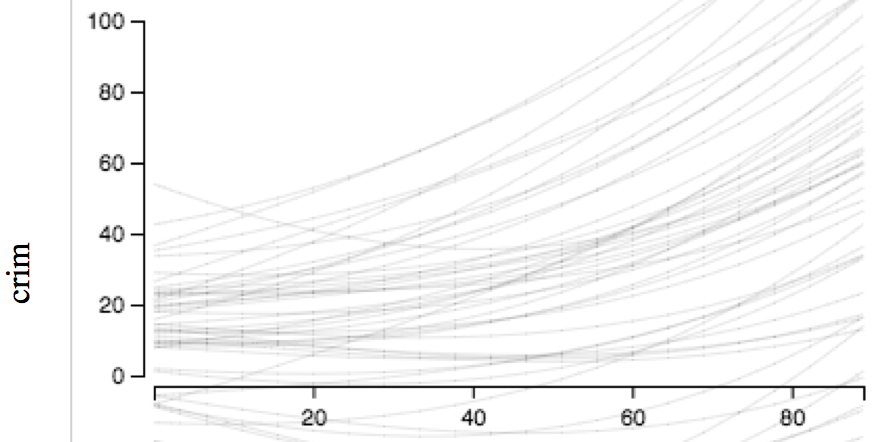
\includegraphics[width=\textwidth]{boston_svm_poly_slices.png}
      \caption{
      }
      \label{fig:nn_slices:f}
    \end{subfigure}
    &
    \begin{subfigure}[b]{0.2\textwidth}
      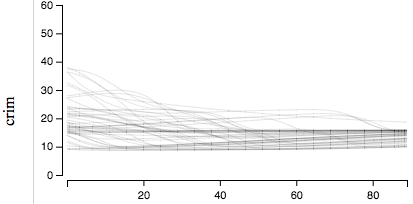
\includegraphics[width=\textwidth]{boston_nn_5x3_slices_zoomed.png}
      \caption{
      }
      \label{fig:nn_slices:g}
    \end{subfigure}
    &
    \begin{subfigure}[b]{0.2\textwidth}
      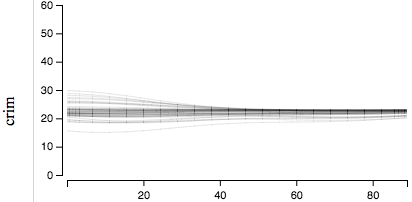
\includegraphics[width=\textwidth]{boston_svm_radial_slices_zoomed.png}
      \caption{
      }
      \label{fig:nn_slices:h}
    \end{subfigure}
  \end{tabular}
  \caption{
    Two different views of the predictions of four different machine learning
    regression models on the Boston housing dataset. The top row (a -- d) shows
    predictions by each model compressed to two dimensions with t-SNE. We
    colored the points on a continuous color scale with dark blue being 0 and
    light blue the highest value. The bottom row (e -- h) shows a 1D slice view
    of the first dimension of the dataset, crime rate. We show the slices of
    the remaining dimensions in the supplemental material. 
    The 1D slices reveal interesting information about how the models perform and
    can assist with model selection. We may not want to use the SVM with
    polynomial kernel (f), for example, since it predicts that home price will go
    up with higher crime rates.
  }
  \label{fig:nn_comp}
\end{figure*}

%\msnote{sounds a bit too defensive. Deep Learning is the big hype at the moment but nobody understands them! That's imho the core message that we need to say}
Artificial neural networks are currently gaining a lot of attention in machine
learning.  The goal of these algorithms is to produce a multi-dimensional
function fitted to the training points. Neural networks, in particular, have
proven to be very good at producing accurate, generalizable predictions. One of
the major challenges for designers of such models, however, is to properly
architect these networks. For instance, how many hidden layers does one need
and how many nodes should be put into each layer? These architectural choices
can drastically change the predictions.
While these choices are crucial, currently, there is only
little guidance available for designers. A typical rule of thumb is to
use a hidden layer two times the size of the input dimensions.
% or two layers with \ttwnote{some reduction}. 
There are also some general proofs regarding what type of functions neural
networks can represent~\cite{Hornik:1989,Eldan:2016}. However, there are no
formal guidelines for designing these networks~\cite{Goodfellow:2016} and the
way these models make predictions is still obtuse.

One of the ways we can increase the understandability of neural network
regression models is by viewing the response function
directly~\cite{gleicher:2016}. If we want to understand how the network
architecture affects the prediction we could compare the prediction manifold to
one produced by a ``simpler'' machine learning model~\cite{Ribeiro:2016a}, for
example a support vector machine~\cite{Smola:2004}.  Support vector machines
have known guarantees on error rate with the number of training samples. With
this comparison we may be able to get some better insight about how the neural
network learning algorithms are performing.

To compare, we chose the Boston housing dataset~\cite{Lichman:2013} from the
UCI repository. This dataset contains median home prices
given 13 factors including crime rate, age of the house, and proximity to
highways. We then trained a neural network with a single hidden layer of 26
nodes, a neural network with 2 hidden layers: one of 5 and one of 3 nodes, a
support vector machine with a polynomial kernel, and a support vector machine
with a radial (Gaussian) kernel.
%\msnote{Ok, add more detailed notes ... I think the challenge is to add a
%couple of subclauses explaining the ML background in a nutshell and connect it
%to / make its relevance for the problem at hand clear (abstractly, we would
%like to look at and understand multi-D respose surfaces, i.e. multi-D
%continuous functions. As soon as we can see these functions, we also can
%compare different models. That is, if models have similar response surface
%functions, we can use the easier to understand one to as a ``surrogate'' to
%better understand the behavior of the more complex ones ... just some thoughts
%in my words, not sure if this is actually what we want to achieve, but our
%goals should be very clear here ... Said all that, to me I think it is mostly
%clear what you mean, but I might be biased here as I do know our project well
%and can fit in all the pieces without any problem.  ... old: for the above
%paragraphs: need to be explained more clearly imho.  Specifically, they should
%also make the issues and concepts clear to someone who is not necessarily an
%ML expert. Needs re-writing; happy to discuss to give some ideas on what a
%good level of information would be here.}

We compare 1D slices with an adaption of the common way of viewing
classification algorithms to continuous data.
% to maintain \ttwnote{ecological validity?}. 
The results of \emph{classification} models are commonly visualized
by using MDS~\cite{Kruskal:1964} or t-SNE~\cite{Maaten:2008} to reduce the input
dimensions to two and then present a scatterplot with the predictions colored
by class. We extended this by sampling the prediction model with \(1,000\)
samples from a Latin hypercube~\cite{Tang:1993} (a space-filling design)
converting the points to two dimensions with t-SNE and then coloring the points
on a continuous scale which we show in \autoref{fig:nn_comp} (top row).  The
bottom row of the figure shows the 1D slice view of the same four prediction
models. We only show the first dimension due to space reasons. The full 13
dimension slice view image in \autoref{app:sliceplorer_ml} 
\ttwnote{move image here?}.

Showing the changes in home price as it corresponds directly to the crime rate
can help to increase confidence in a model.  From the prediction lines, one may
not want to use the SVM with a polynomial kernel. By and large the prediction
lines are increasing. This means that the home price is increasing as the crime
rate goes up. This does not really make sense. The model is not generalizing
well. Similarly, the neural network with a single hidden layer (left column)
also has a number of curves that increase as crime increases. The neural
network with two hidden layers does not have this problem. Maybe this is the
best model to use in this case.

%\tmnote{needs a final paragraph, maybe sth like} 
In summary, this usage scenario illustrated that a direct inspection of a
model's response surfaces can give intuition of its behavior, and can lead to a
better model selection and a better intuition of the modeling process. 1D
slices can help to gain important insights in this process. 
%Hence, this type of analysis is not only novel but also insightful.

\subsection{Optimization algorithm}
\label{sec:optimization}

General purpose optimization algorithms try to find the global minimum (or
equivalently, the global maximum) of a function of arbitrary dimension.  Many
optimization algorithms such as Nelder-Mead~\cite{Nelder:1965} work by starting
at a particular parameter setting and evaluating the ``shape'' of the function
around that point.  The algorithm then determines where the function is
decreasing the greatest, and ``jumps'' a certain distance in that direction.
The ``jump'', starting position, and termination tolerance parameters are
user-settable parameters. Depending on how they are set, the algorithm can get
stuck in a local minima or take unreasonably long to finish.

When one is trying to parameterize or build optimization algorithms then
one wants to evaluate the trace of the optimization on an easy function
that is fast to compute first. This analysis helps to better understand how to parameterize for more complex problems
%, which will be faced in reality, 
but are
too computationally expensive to analyze directly. 
Visual inspection of the easy function before running the optimization algorithm, as well as
viewing the trace of the optimization algorithm (the sequence of steps it took) is a good way to ensure that the algorithm is converging towards the global
minimum. 
%\msnote{... maybe something: you would also like to use the algorithm
%inn other situations as well or so?}\ttwnote{not sure what you mean}
%\msnote{... old: just playing devil's advocate: So, we have the visual minimum,
%why care about the visualization then if you simply could compute a number
%between the visual global minimum and the algorithmically detected minimum}
%\msnote{TO DISCUSS: what about a number for the difference between the visual minimum in the slices and 
%the local minimum found?}
%\msnote{TO DISCUSS: also, how would the other alternatives perform here?}

We compare 1D slices with HyperSlice~\cite{Wijk:1993} as this is the only
technique that also directly visualizes the parameter space.  We ran the
Nelder-Mead optimization algorithm on the 5D Ackley
function~\cite{Ackley:1987}, a popular optimization algorithm testing function.
To examine the effect of starting position, we tried different starting
positions: \(x=(1,1,1,1,1)\) and \(x=(2,2,2,2,2)\).  We overlay the
optimization trace on top of both 1D slices and HyperSlice and the results are
shown in \autoref{fig:optim_trace}.

\begin{figure}
  \centering
  \begin{subfigure}[b]{0.35\linewidth}
    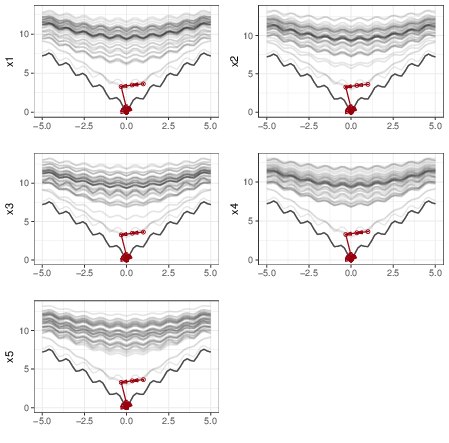
\includegraphics[width=\textwidth]{optim_trace_1_1.png}
    \subcaption{ 
      \label{fig:optim_1:sp}
    }
  \end{subfigure}
  \qquad\qquad
  \begin{subfigure}[b]{0.35\linewidth}
    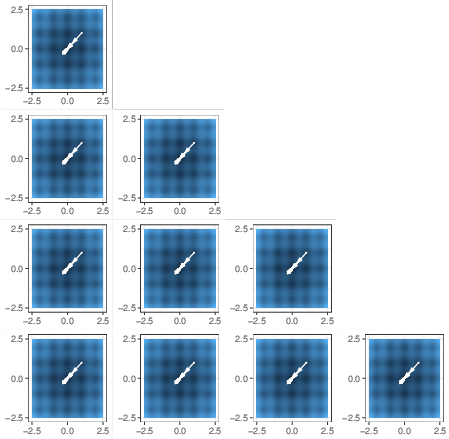
\includegraphics[width=\textwidth]{optim_trace_hs_1_1.png}
    %\resizebox{\textwidth}{!}{%
    %\begin{tabular}{rrrrr}
      %20.9885770  & -0.3256642 & -0.3257547 & -0.3258958 & -0.3252083 \\
      %-0.3256642  & 20.9908910 & -0.3254367 & -0.3255775 & -0.3248914 \\
      %-0.3257547  & -0.3254367 & 20.9902343 & -0.3256679 & -0.3249814 \\
      %-0.3258958  & -0.3255775 & -0.3256679 & 20.9892087 & -0.3251219 \\
      %-0.3252083 & -0.3248914 & -0.3249814 & -0.3251219 & 20.9941950
    %\end{tabular}
    %}
    \subcaption{
      \label{fig:optim_1:hs}
    }
  \end{subfigure}
  \\
  \begin{subfigure}[b]{0.35\linewidth}
    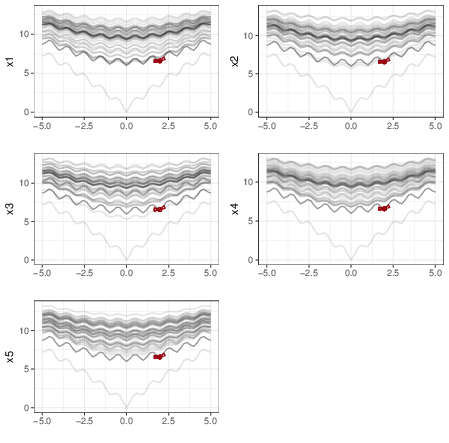
\includegraphics[width=\textwidth]{optim_trace_2_1.png}
    \subcaption{
      \label{fig:optim_2:sp}
    }
  \end{subfigure}
  \qquad\qquad
  \begin{subfigure}[b]{0.35\linewidth}
    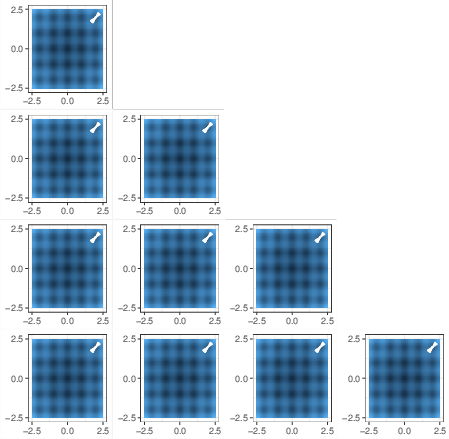
\includegraphics[width=\textwidth]{optim_trace_hs_2_1.png}
    %\resizebox{\textwidth}{!}{%
    %\begin{tabular}{rrrrr}
      %21.0042955 & -0.1840739 & -0.1843067 & -0.1846840 & -0.1845613 \\
      %-0.1840739 & 21.0067633 & -0.1839595 & -0.1843355 & -0.1842132 \\
      %-0.1843067 & -0.1839595 & 21.0051112 & -0.1845689 & -0.1844464 \\
      %-0.1846840 & -0.1843355 & -0.1845689 & 21.0024265 & -0.1848241 \\
      %-0.1845613 & -0.1842132 & -0.1844464 & -0.1848241 & 21.0033008
    %\end{tabular}
    %}
    \subcaption{
      \label{fig:optim_2:hs}
    }
  \end{subfigure}
  \caption{
    1D slice and HyperSlice views showing
    traces of an optimization algorithm searching for the global minimum
    of a 5D Ackley function.
    (\subref{fig:optim_1:sp}) and 
    (\subref{fig:optim_1:hs}) show the trace starting at the point
    $(1,1,1,1,1)$ while 
    (\subref{fig:optim_2:sp}) and 
    (\subref{fig:optim_2:hs}) 
    show the trace starting at the point $(2,2,2,2,2)$. 
  }
  \label{fig:optim_trace}
\end{figure}

The 1D slice view allows us to see the path that the algorithm took and the
general shape of the function simultaneously.  In addition, the 1D slice view
shows that the distribution of values around the global minimum is small. Most
of the slices are clustered around \(y=10\) with only one slice descending
close to \(y=0\). Since the sampling is uniform in the parameter space this
means that it is very difficult to select slices around the global minimum. In
fact, this is a known property of the Ackley function.  It is easy to see that
the optimization algorithm got stuck at a local minimum when started at
\(x=(2,2,2,2,2)\). However, with the HyperSlice view it is difficult to see the
difference in value and steepness of the function at \(x=(1,1,1,1,1)\) versus
\(x=(2,2,2,2,2)\).  Humans are not good at perceiving fine differences in
color~\cite{Munzner:2014}, but is required for this task. We learn a lot more
about the behavior of the optimization algorithm from the 1D slice views (see
\autoref{fig:optim_1:sp} and \autoref{fig:optim_2:sp}) than the HyperSlice
view. However, the HyperSlice view does clearly show that that optimization
algorithm is moving in multiple directions at once. This is not clear in the 1D
slice views.




\section{Discussion}

The above examples illustrated that the technique of 1D slices as presented are
quite flexible and useful for various low- and high-level tasks.  However, I do
not intend to claim that it is the only and best method for all problems out
there. Rather, I would like to argue that it is a valuable (and thus far
overlooked) technique in a toolbox of visual inspection methods for
multi-dimensional functions. I hope that this work inspires a discussion and
exploration of guidelines for tasks, proper visual encoding, and interaction
techniques for various application areas. Along these lines I would like to put
forth our current experience with various techniques.

\textbf{Topological techniques are helpful for a global overview}: Topological
techniques allow us to compare \emph{between} optima but are not as good at
evaluating the area \emph{around} an optimum since these areas are typically
abstracted away.  Topological spines attempts to compensate for this by showing
the area covered by a particular optimum as an area around the node. However,
many of the tasks like ``correlate'' and ``cluster'' are best served by viewing
the response manifold directly. In a larger system, the topological techniques
could be used effectively as a global overview of the function with a
HyperSlice or 1D slice showing local context. Selecting a point in the
topological view would change the focus point in the local view.

\textbf{HyperSlice is good when you need to show 2D interactions}: HyperSlice
is the only technique that can display more than one dimension of data
interaction.  So, if this is a requirement then HyperSlice is the best option.
However, one can use 1D slices to get a general overview of the dependence of
the function on each dimension. The dimensions that are not interesting
because, for example, the function is not sensitive to them could easily be
eliminated from further consideration. This would reduce the number of subplots
that we need to view in the HyperSlice plot.

\textbf{1D slices should be used for a ``first pass'' visualization}: 1D slices
addresses many of the tasks that a user wants to perform. The technique does a
very good job on a wide variety of tasks. 1D slices are easy to
implement, easy to understand, and the static view provides a lot of
information.


\section{Limitations and future work}
%\label{sec:limitations}

The 1D slice view consists of a projection of many lines.  the distribution of
slices are shown through direct projection. Techniques like contour
boxplots~\cite{Whitaker:2013} and curve boxplots~\cite{Mirzargar:2014} build a
distribution model of curves which could help to address the ``characterize
distribution'' task in \autoref{tbl:task_list}. However, neither of these or
any of the other time curve visualization techniques have been applied to
multi-dimensional functions. Evaluating these techniques for this purpose is an
exciting topic for future work.

When developing the 1D continuous slicing technique I only considered
multi-dimensional continuous scalar functions in terms of requirements, 
tasks, and comparisons. I do not consider multi-field 
(i.e.\ functions with multiple outputs) or complex-valued functions in the
analysis. There are multi-field topology techniques to address 
this~\cite{Duke:2012,Huettenberger:2014,Carr:2015} which I do not consider
but the technique and analysis would need to be extended to this domain.
This is left for future work.

The x-axis of each 1D slice is independent of the x-axes of the other 1D
slices. This allows each plot to scale individually if the range of inputs have
different values.  The x-axis and y-axis automatically change to incorporate
their respective minimum and maximum ranges. While the x-axis scales itself
independently, the y-axis is the same for each plot.  This is also the default
behavior in many of-the-shelf plotting packages. The plots will adjust
automatically to shifts.  For the x-axis we use axis-aligned projections.
Therefore, the views are sensitive to rotational transformations of the
function. 

Finally, the Sliceplorer technique is also based on sampling, just like the 
techniques used in the comparison.
As with any technique based on sampling one
must be careful to take an adequate number of samples in order to properly
capture all desired behavior.
%\ttwnote{add more about sampling limitations?}
If the function is not smooth we may see a slice that is an ``outlier,'' i.e.\
one slice is much higher or lower than all the others. In this case all other
slices will be compressed into either the top or bottom of the chart. This is
often a problem with many common visualization techniques like bar graphs or
scatterplots and can be addressed with log scaled axes, for example.



Understanding multi-dimensional spaces is difficult. Visualization can give
us context to help understand the geometry. With the direct visualization
of these multi-dimensional continuous datasets through slice views, we can
use a familiar concept to give context and meaning to a complex task.

Multi-dimensional continuous functions are commonly visualized with 2D slices
or topological views. With Sliceplorer, I explore 1D slices as an alternative
approach to show such functions. My goal with 1D slices is to combine the
benefits of topological views, that is, screen space efficiency, with those of
slices, that is a close resemblance of the underlying function.  I compare 1D
slices to 2D slices and topological views, first, by looking at their
performance with respect to common function analysis tasks. I also demonstrate
3 usage scenarios: the 2D sinc function, neural network regression, and
optimization traces. Based on this evaluation, I characterize the advantages
and drawbacks of each of these approaches, and show how interaction can be used
to overcome some of the shortcomings. 


I also presented Hypersliceplorer, an algorithm for generating 2D
slices of multi-dimensional shapes defined by a simplical mesh.  Often, slices
are generated by using a parametric form and then constraining parameters to
view the slice. In this case, I developed an algorithm to slice a simplical
mesh of any number of dimensions with a two-dimensional slice. In order to get
a global appreciation of the multi-dimensional object, I show multiple slices
by sampling a number of different slicing points and projecting the slices into
a single view per dimension pair. These slices are shown in an interactive
viewer which can switch between a global view (all slices) and a local view
(single slice). I show how this method can be used to study regular polytopes,
differences between spaces of polynomials, and multi-objective optimization
surfaces. 


Finally, I develop a method for predicting the rendering time to display
multi-dimensional data for the analysis of computer simulations using the
HyperSlice~\cite{Wijk:1993} method with Gaussian process model reconstruction.
My method relies on a theoretical understanding of how the data points are
drawn on slices and then fits the formula to a user's machine using practical
experiments.  I also describe the typical characteristics of data when
analyzing deterministic computer simulations as described by the statistics
community.  I then show the advantage of carefully considering how many data
points can be drawn in real time by proposing two approaches of how this
predictive formula can be used in a real-world system.


\subsection{Future}

My work has had a major focus on using direct visualization techniques to
understand multi-dimensional continuous spaces. My intention is that this work
can be expanded upon to herald in a new era of multi-dimensional data analysis.
In my opinion, the major innovations preventing this technique from being used
in a broader application are a library for slicing multi-dimensional spaces and
more user-focused projects.  Building on these two thrusts will move
multi-dimensional continuous data analysis to the mainstream.

One of the reasons for the lack of adoption for slice-based visualization of
multi-dimensional objects is the complete lack of software to generate even
static slice views. There are many libraries for popular data analysis
languages like Python, Javascript, and R. In order to make slice based views
more viable I plan to develop an interactive slice-based visualization software
based on the prototype tools I have already developed. This will lower the cost
of entry of slice-based views of multi-dimensional continuous datasets. The end
result is more users familiar with this visualization type.

In addition, more focused projects with end-users in the form of design
studies~\cite{Sedlmair:2012} will help to develop both the task taxonomy and
the visualization techniques. As part of the task abstraction, we can learn how
these users' tasks fit in with the task and data taxonomy proposed in this
thesis. Then we can refine and extend the task and data taxonomy. This taxonomy
will allow visualization researchers to identify gaps and develop tools to
address them, thus creating more effective visualizations of multi-dimensional
continuous data.


\subsection{Implications}

The main goal of my thesis was to explore what is possible with slice-based
visualizations of continuous multi-dimensional datasets. My hope is that this
work will serve as a basis for an increasing focus on direct visualization of
multi-dimensional objects. Often it seems that the default analysis technique
for more than three dimensions is to reduce
the dimensionality of the
data and then render the reduced data on screen. This suffers from issues of
distortion of distances and relative sizes. The analysis tasks for
multi-dimensional data are all developed around understanding the carefully
chosen dimensions. Hence, transforming these dimensions takes away a lot of
contextual knowledge about the simulation. 

I also hope to bring more attention to continuous multi-dimensional data analysis.
In the visualization community, most of the work on multi-dimensional and high-dimensional
data has focused on the discrete case. There are many task taxonomies, techniques,
and applications for discrete data. My hope with this thesis is that by developing
a task and data taxonomy as well as an in-depth study of direct visualization
techniques will bring similar attention to multi-dimensional continuous data
analysis. There are a number of under-explored application areas in this
field. I have identified some in my own work, but with further research in this
field will bring more knowledge and understanding about how we, as three-dimensional
beings can understand multi-dimensional continuous datasets.







